%            PACKAGES AND OTHER DOCUMENT CONFIGURATIONS
%----------------------------------------------------------------------------------------
\documentclass[paper=letter,11pt]{article}
\usepackage[spanish]{babel} 
\decimalpoint
\usepackage{amsmath,amsfonts,amsthm} % Math packages
\usepackage{floatrow}
\usepackage{subfig}
\captionsetup[subfigure]{labelformat=simple, labelsep=none}
\renewcommand{\thesubfigure}{\alph{subfigure})}
\usepackage[utf8]{inputenc}
\usepackage{float}
\usepackage{lipsum} % Package to generate dummy text throughout this template
\usepackage{blindtext}
\usepackage{graphicx} 
\graphicspath{{Figuras/}} % Directory in which figures are stoorange
\usepackage[font=footnotesize,labelfont=bf]{caption}
\usepackage{subcaption}
%\usepackage{cmr} % Use the Palatino font
\usepackage{lmodern}
\usepackage[T1]{fontenc} % Use 8-bit encoding that has 256 glyphs
\linespread{1.05} % Line spacing - Palatino needs more space between lines
\usepackage{microtype} % Slightly tweak font spacing for aesthetics
\usepackage[hmarginratio=1:1,top=32mm,columnsep=20pt]{geometry} % Document margins
\usepackage{multicol} % Used for the two-column layout of the document
%\usepackage[hang, small,labelfont=bf,up,textfont=it,up]{caption} % Custom captions under/above floats in tables or figures
\usepackage[figurename=Fig.]{caption}
\usepackage{booktabs} % Horizontal rules in tables
\usepackage{float} % Required for tables and figures in the multi-column environment - they need to be placed in specific locations with the [H] (e.g. \begin{table}[H])
\usepackage{hyperref} % For hyperlinks in the PDF
\usepackage{wrapfig}
\usepackage{xcolor}
\usepackage{lettrine} % The lettrine is the first enlarged letter at the beginning of the text
\usepackage{paralist} % Used for the compactitem environment which makes bullet points with less space between them
\usepackage{abstract} % Allows abstract customization
\renewcommand{\abstractnamefont}{\normalfont\bfseries} % Set the "Abstract" text to bold
\renewcommand{\abstracttextfont}{\normalfont\small\itshape} % Set the abstract itself to small italic text
\usepackage{titlesec} % Allows customization of titles



\renewcommand\thesection{\Roman{section}} % Roman numerals for the sections
\renewcommand\thesubsection{\Roman{subsection}} % Roman numerals for subsections
\newcommand{\uvec}[1]{\hat{e}_{#1}}

\titleformat{\section}[block]{\large\scshape\centering}{\thesection.}{1em}{} % Change the look of the section titles
\titleformat{\subsection}[block]{\large\bf}{\thesubsection.}{1em}{} % Change the look of the section titles
\newcommand{\horrule}[1]{\rule{\linewidth}{#1}} % Create horizontal rule command with 1 argument of height

\usepackage{physics}
\usepackage[bibstyle = trad-abbrv,
citestyle = numeric-comp,
backend = bibtex, 
sorting = none, % Sort as they appear
backref=true]{biblatex} %style = trad-abbrv 
\AtEveryBibitem{\clearfield{urldate}}
\AtEveryBibitem{\clearfield{url}}
\AtEveryBibitem{\clearfield{isbn}}
\AtEveryBibitem{\clearfield{month}}
\AtEveryBibitem{\clearfield{day}}
\AtEveryBibitem{\clearfield{issn}}
\DeclareFieldFormat[article]{volume}{\mkbibbold{#1}}
\addbibresource{Referencias.bib}
%cambiar a negrita los numeros de las ecuaciones
%\makeatletter
%\def\tagform@#1{\maketag@@@{(\ignorespaces\textbf{#1}\unskip\@@italiccorr)}}
%\renewcommand{\eqref}[1]{\textup{{\normalfont(\ref{#1}}\normalfont)}}
%\makeatother

%---------------------------------------------------------------------------------------
%IMÁGENES INCLUIDAS


%----------------------------------------------------------------------------------
\hypersetup{colorlinks=true,linkcolor=blue,citecolor=blue,filecolor=blue,urlcolor=magenta}

\usepackage{fancyhdr} % Headers and footers
\pagestyle{fancy} % All pages have headers and footers
\fancyhead{} % Blank out the default header
\fancyfoot{} % Blank out the default footer
\fancyhead[RO,LE]{Universidad Nacional Autónoma de México | Facultad de Ciencias | Servicio Social } % Custom header text
\renewcommand{\headrulewidth}{0.4pt}

\fancyfoot[RO,LE]{\thepage} % Custom footer text
\fancyheadoffset[RO,LE]{0.01\textwidth}


%----------------------------------------------------------------------------------------
%       TITLE SECTION
%----------------------------------------------------------------------------------------
\title{\vspace{-15mm}\fontsize{17pt}{1.25em}\selectfont\textbf{Cálculo de las secciones transversales de extinción, absorción y esparcimiento de elipsoides en la aproximación cuasiestática como primera aproximación de eritrocitos }} % Article title
\author{
\large
{\textsc{ Dana Larissa Luna González}}\\[2mm]}
\date{}
\geometry{total={170mm,230mm}, left=20mm, top=25mm}

 
 
\begin{document}
\maketitle % Insert title
\thispagestyle{fancy} % All pages have headers and footers
\floatsetup[figure]{style=plain,subcapbesideposition=top}


\section{Introducción}
El estudio de las propiedades ópticas de las células biológicas como los osteoblastos \cite{Osteoblastos}, los linfocitos \cite{Linfocitos}, y los eritrocitos \cite{Blood}, es de importancia para el área médica. A partir de las propiedades ópticas de las células, se obtiene información de su composición y estado morfológico, lo cual tiene potenciales aplicaciones en el diagnóstico y la detección temprana de diversas enfermedades, incluidos cánceres e infecciones virales \cite{Linfocitos}. En particular, el estudio de los eritrocitos tiene un papel importante en el diagnóstico de la anemia en sus diferentes tipos y el diseño de nuevas terapias ópticas, como el tratamiento de las venas varicosas \cite{Blood}. \\

Los eritrocitos sanos presentan forma de discoides cóncavos con longitudes de entre 4 a 9 $\mu$m de diámetro. Estos no poseen núcleo, por lo que pueden modelarse como un objeto homogéneo \cite{Cassini}. Debido a su forma, para simplificar el proceso de modelado, se han empleado diferentes opciones como los óvalos de Cassini \cite{Cassini} o funciones en términos de coordenadas esféricas \cite{Esferico}. Sin embargo, una primera aproximación es considerarlos como un elipsoide. El objetivo éste trabajo es el de analizar la respuesta óptica de elipsoides de diferentes materiales (oro, plata, aluminio, bismuto y óxido de magnesio) y tamaños dentro de la nanoescala, por medio de las secciones transversales de esparcimiento, absorción y extinción, bajo la aproximación cuasi-estática para, posteriormente, orientarlo a eritrocitos. En la \hyperlink{primera}{Sección I} de éste trabajo, se resuelve de forma analítica el problema de esparcimiento de luz por una partícula elipsoidal arbitraria en la aproximación cuasiestática, donde se presentan, además, las secciones transversales de extinción, absorción y esparcimiento. En la sección de \hyperlink{resultados}{Resultados}, se estudia el esparcimiento de luz por un elipsoide centrado en el origen, en la aproximación cuasi-estática para partículas elipsoidales oblatas de materiales tanto plasmónicos como dieléctricos. Finalmente, en la sección de \hyperlink{conclusiones}{Conclusiones}, se presenta un resumen de lo estudiado en éste trabajo, así como los principales resultados obtenidos.




\hypertarget{primera}{\subsection{Aproximación cuasiestática en el problema de esparcimiento de luz por partículas elipsoidales}}

 En el caso de un elipsoide de semieje mayor $a$ caracterizado por una función dieléctrica $\epsilon_p$, inmerso en un medio con una función dieléctrica $\epsilon_m$, e iluminado por una onda plana electromagnética con vector de onda $\Vec{k}$, se puede definir el límite cuasiestático cuando el parámetro de tamaño $x=ka$ es mucho menor que la unidad \cite{Bohren}. Ésta constricción garantiza que toda la geometría del elipsoide esté sujeta a un campo eléctrico de la misma intensidad y dirección \cite{Cuasiestatico}. En ésta sección se presenta el caso de una esfera, como caso particular de un elipsoide, en el límite cuasiestático para estudiarlo como un dipolo eléctrico puntual, lo que permite introducir el concepto de polarizabilidad, y más adelante, se desarrolla el dipolo eléctrico para esparcidores arbitrarios en donde se analizan las regiones de campo cercano, intermedia y de radiación.


\subsubsection{Dipolo eléctrico (caso estático)}

En electrodinámica clásica, se entiende como \textit{límite cuasiestático} el considerar una partícula de tamaño mucho menor que la longitud de onda de la luz incidente \cite{Cuasiestatico}. Para el caso de una partícula esférica de radio $a$, se puede emplear la aproximación cuasiestática al resolver la ecuación de Laplace para el potencial eléctrico $\phi$. Si se considera una esfera con permitividad eléctrica $\epsilon_p$, embebida en un medio caracterizado por su función dieléctrica $\epsilon_m$ en el cual existe un campo eléctrico externo $\Vec{E}_0=E_0\hat{e}_z$ [Fig. \ref{system}], al resolver la ecuación de Laplace considerando las condiciones de frontera entre la esfera y el medio, se obtiene que el potencial eléctrico fuera de la esfera es la superposición del campo eléctrico aplicado y del campo eléctrico producido por un dipolo eléctrico puntual $\vec{p}$ localizado en el origen. El potencial eléctrico correspondiente al campo eléctrico producido por el dipolo eléctrico puntual está dado por \cite{Griffiths}
\begin{equation}
	\phi_p(\vec{r}\,)=\frac{p}{4\pi\epsilon_m}\left(\frac{\Vec{r}\cdot\hat{e}_z}{r^3}\right)=\frac{\Vec{p}\cdot\Vec{r}}{4\pi\epsilon_m r^3}=\frac{p\cos\theta}{4\pi\epsilon_m r^2},
	\label{pot_dipolo}
\end{equation}
donde $\Vec{p}$ representa el momento dipolar eléctrico expresado como \cite{Bohren}
\begin{equation*}
	\vec{p}= \epsilon_m\alpha\Vec{E}_0=4\pi\epsilon_m a^3\left(\frac{\epsilon_p-\epsilon_m}{\epsilon_p+2\epsilon_m}\right)\Vec{E}_0, \;\:\:\:\:\: \text{con}\; \alpha=4\pi a^3\left(\frac{\epsilon_p-\epsilon_m}{\epsilon_p+2\epsilon_m}\right), 
	\label{momentdipol}
\end{equation*}
donde $\alpha$ es la polarizabilidad eléctrica, que representa la facilidad con la que se polariza la esfera, es decir, el campo eléctrico externo induce un dipolo eléctrico puntual en la esfera, cuyo campo eléctrico asociado fuera de la esfera es 
\begin{equation*}
	\Vec{E}_p(\vec{r}\,)=-\nabla \phi_p =\frac{p}{4\pi \epsilon_m r^3 }\left(2\cos\theta\hat{e}_r+\sen\theta\hat{e}_{\theta}\right).
\end{equation*}
En consecuencia, el campo eléctrico fuera de la esfera está dado por la superposición del campo eléctrico externo aplicado y del campo eléctrico externo producido por el dipolo eléctrico [ver Fig. \ref{electricfieldsphere}].


\begin{figure}[H]
	\centering
		\sidesubfloat[First image]{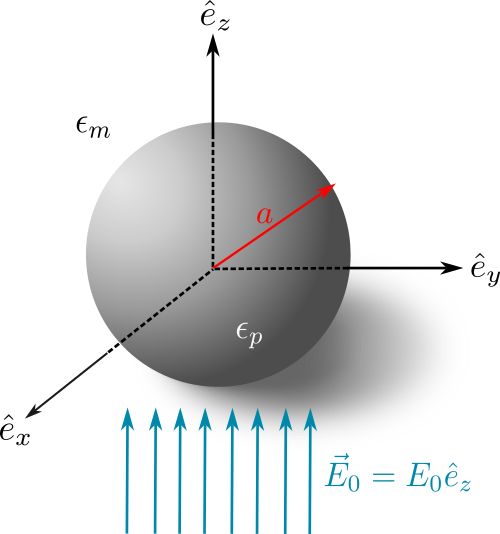
\includegraphics[width=0.3\textwidth]{../../Figuras/shereE0}\label{system}}
		\sidesubfloat[Second image]{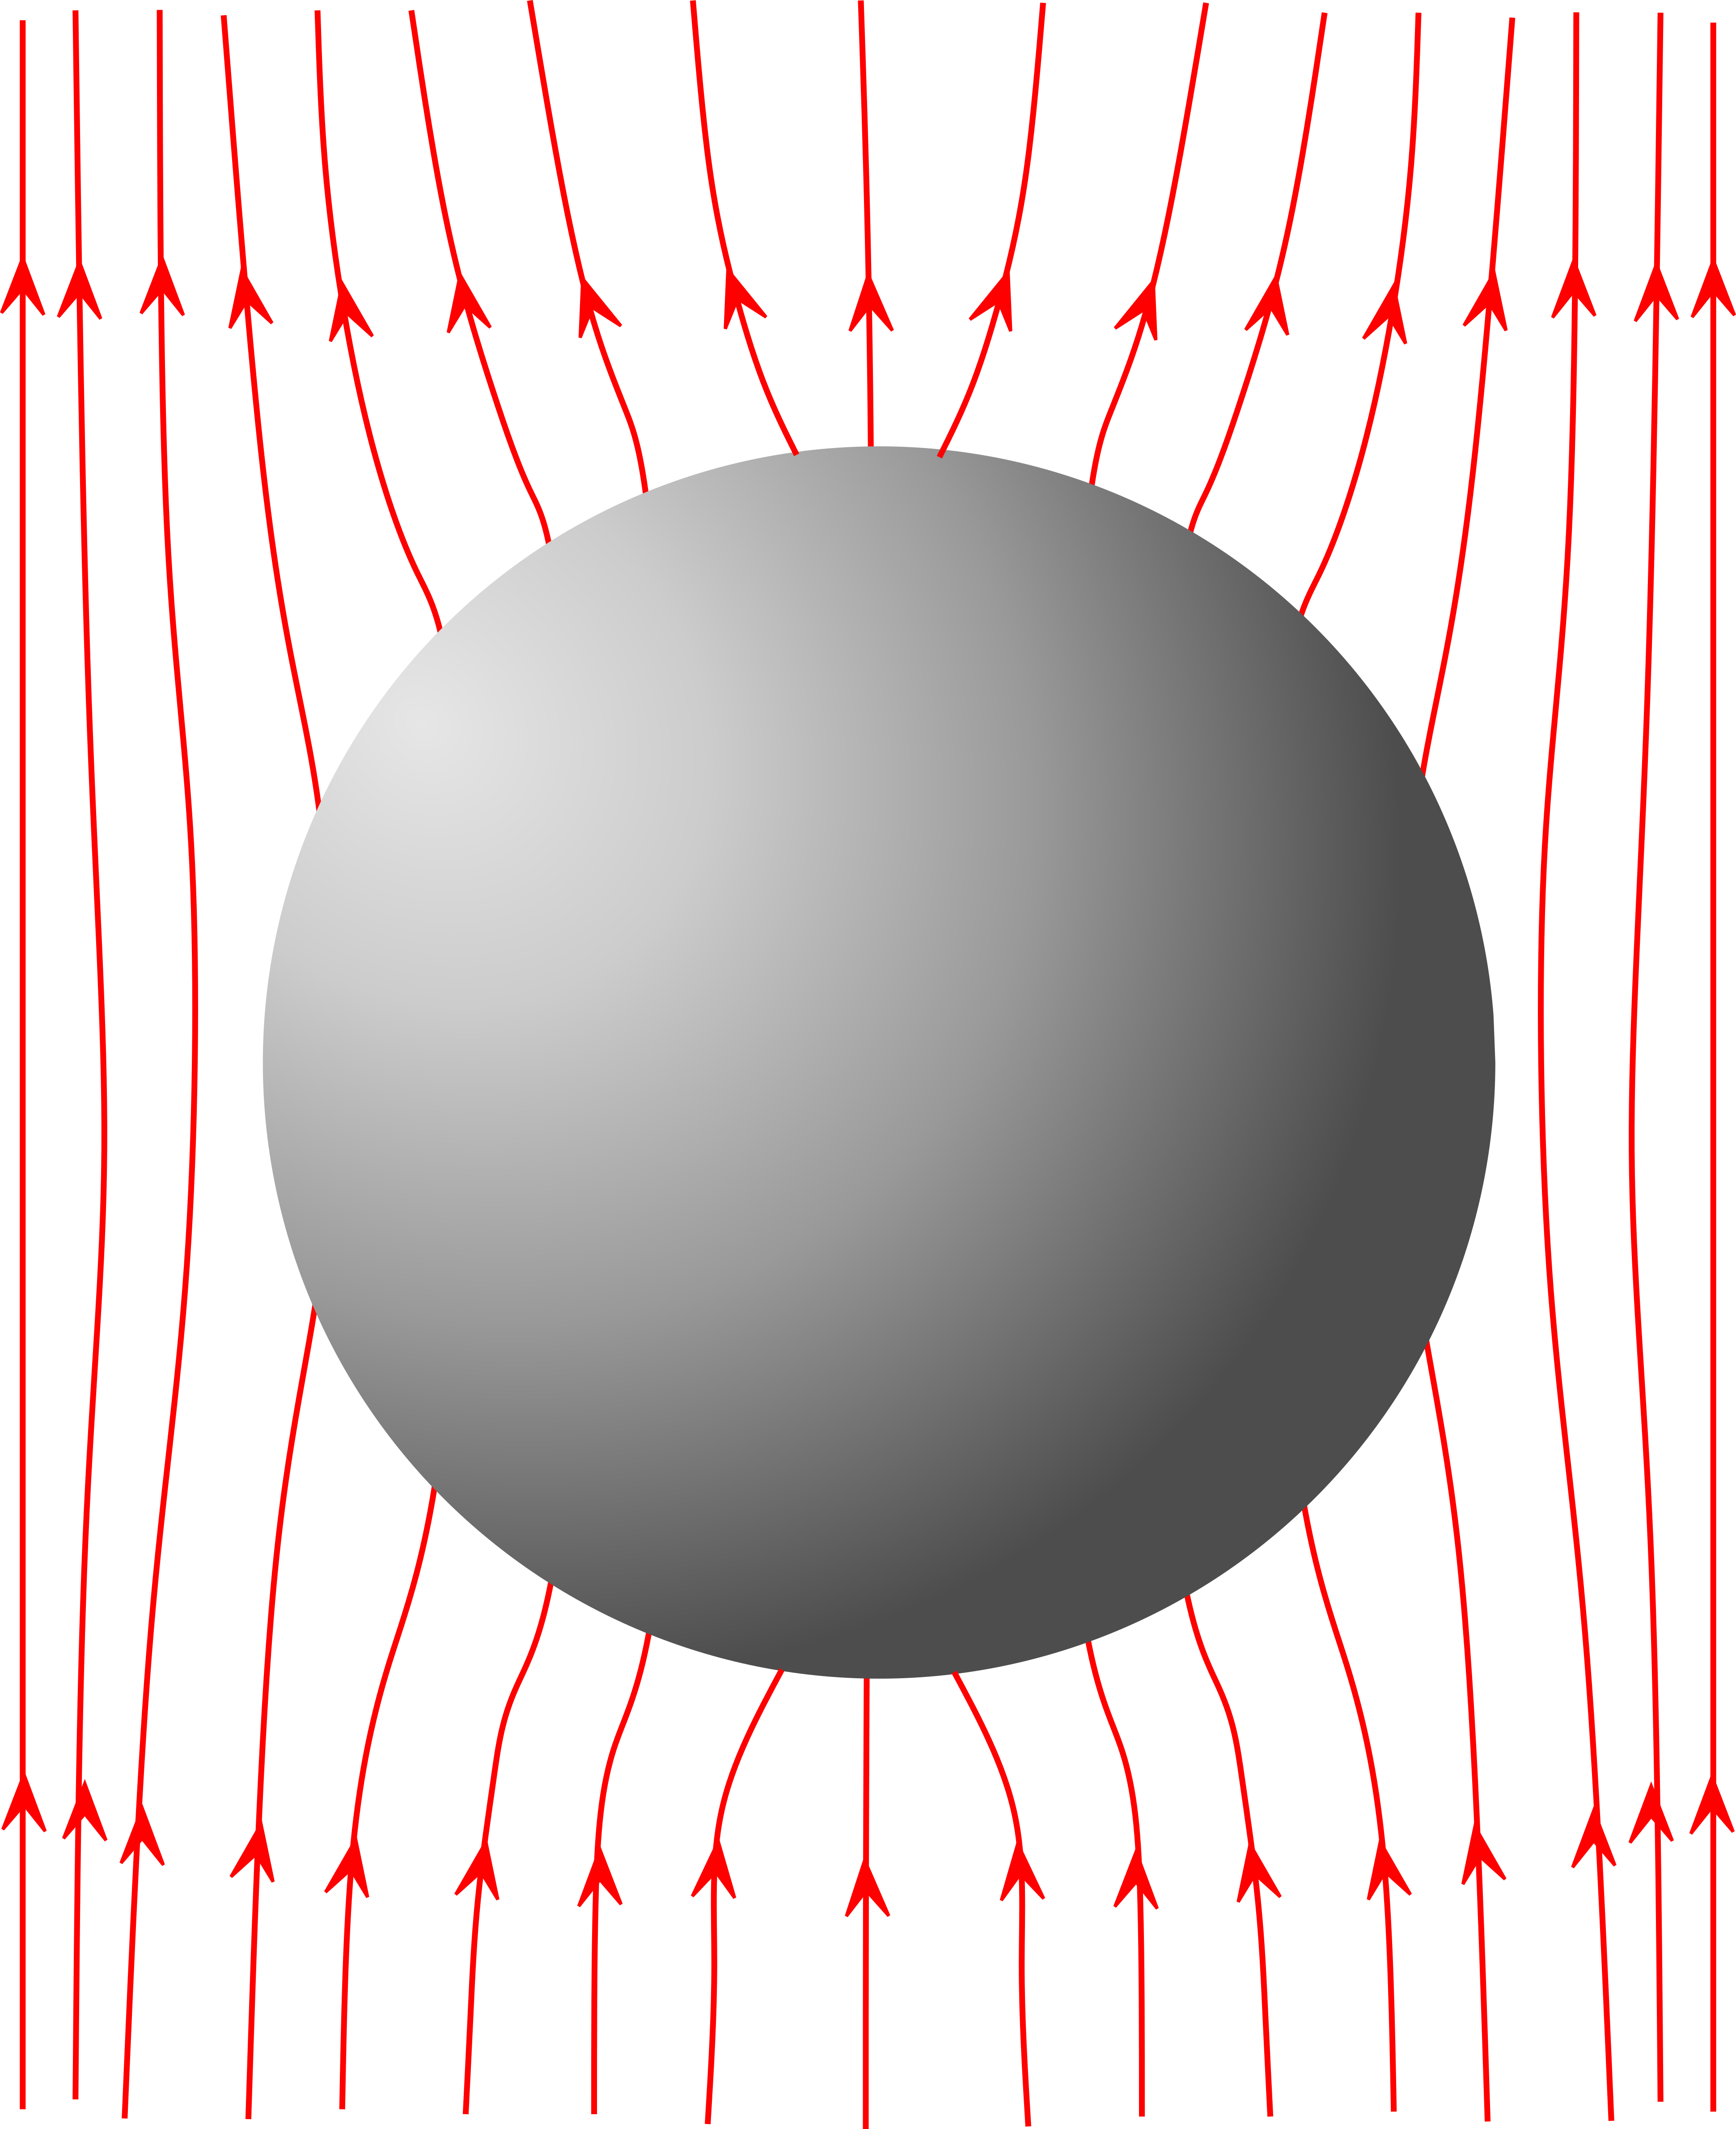
\includegraphics[width=0.25\textwidth]{../../Figuras/electricfield_sphere.png}\label{electricfieldsphere}}
	\caption{Problema de una esfera inmersa en un campo eléctrico homogéneo. \textbf{a)} Esfera de radio $a$ caracterizada por la función dieléctrica $\epsilon_p$ y embebida en un medio caracterizado por la función dieléctrica $\epsilon_m$, en la cual incide un campo eléctrico externo uniforme $\Vec{E}_0$. \textbf{b)} Campo eléctrico fuera de la esfera generado por la superposición del campo eléctrico externo aplicado y del campo eléctrico producido por un dipolo eléctrico puntual localizado en el origen.}
	\label{steady_state}
\end{figure}
 

\subsubsection{Dipolo eléctrico (caso dinámico)}

En la sección anterior se abordó una solución que asume que el campo eléctrico externo, y por tanto también el dipolo inducido, son estáticos. Para resolver el caso dinámico en el régimen cuasiestático, se considera que, al iluminar cargas confinadas en un volumen finito con una onda plana electromagnética, éstas experimentan movimiento al ser sometidas a una fuerza. Esto equivale a realizar un análisis en términos de componentes de Fourier de los potenciales y campos generados por un sistema de cargas y corrientes localizadas en el espacio vacío, con una dependencia armónica $e^{-i\omega t}$, tal que varían en el tiempo y oscilan a la frecuencia $\omega$ del campo electromagnético externo aplicado. De ésta forma, la densidad de carga volumétrica total $\rho(\Vec{r},t)$ y la densidad de corriente volumétrica total $\Vec{J}(\Vec{r},t)$  en la posición $\Vec{r}$ se expresan como \cite{Jackson}
\begin{align}
    \rho(\Vec{r},t)&=\rho(\Vec{r}\,)e^{-i\omega t},\nonumber\\
    \Vec{J}(\Vec{r},t)&=\Vec{J}(\Vec{r}\,)e^{-i\omega t},
    \label{armonicf}
\end{align}
considerando que el significado físico lo posee la parte real. Entonces, es posible determinar los campos electromagnéticos generados por las cargas y corrientes mediante el potencial vectorial como \cite{Jackson}:
\begin{align}
  \Vec{A}(\Vec{r},t)=\frac{\mu_0}{4\pi}\int \left( \text{d}^3r'\frac{\Vec{J}(\Vec{r}\,')}{|\Vec{r}-\Vec{r}\,'|}\right)e^{-i\omega t_r},
  \label{Achafa}
\end{align}
en donde se emplea la norma de Lorentz \cite{Griffiths} y la densidad de corriente se evalúa en el tiempo de retardo $t_r=t-|\Vec{r}-\Vec{r'}|/c$. \\

Al considerar la naturaleza de la onda plana, caracterizada por $\omega$, se pueden definir diferentes regiones de interés. Para estudiarlas, se delimitan en términos de $k=\omega/c$ (o equivalentemente, mediante la longitud de onda $\lambda=2\pi/k$). Por ejemplo, en la región de campo cercano, donde $r\ll\lambda$ (o $kr\ll 1$), tal que exp($ik|\Vec{r}-\Vec{r'}|)\to 1$, se tiene que, al obviar la dependencia temporal, la Ec. (\ref{Achafa}), se reescribe como \cite{Jackson}
\begin{equation*}
	\Vec{A}(\Vec{r}\,)=\frac{\mu_0}{4\pi}\int \frac{\Vec{J}(\Vec{r}\,')}{|\Vec{r}-\Vec{r}\,'|} \text{d}^3r',
\end{equation*} 
mientras que en la región de campo lejano ($kr\gg 1$), dado que la exponencial oscila rápidamente, es suficiente aproximar
\begin{equation}
	|\Vec{r}-\Vec{r}\,'|\simeq r-\hat{e}_r\cdot\Vec{r}\,',    
\end{equation}
 que se obtiene al aplicar la ley de cosenos\footnote{Empleando la ley de cosenos y haciendo una expansión binomial $
 	|\Vec{r}-\Vec{r}\,'|=\sqrt{r^2+r'\,^2-2rr'\cos\theta}=r\sqrt{1+\left(r'/r\right)^2-2\left[(r'/r)\cos\theta\right]}\simeq r\left\{1-(\hat{e}_r\cdot\Vec{r}\,'/r)+1/2\left(r'/r\right)^2\right\}\simeq r-\hat{e}_r\cdot\Vec{r}\,'.$} en el triángulo mostrado en la Fig.~\ref{vectposi}, donde $\hat{e}_r$ un vector unitario en la dirección de $\Vec{r}$. 	
	Si sólo se consideran los términos que decaen como $r^{-1}$, el inverso de la distancia en la Ec. (\ref{Achafa}) puede ser reemplazado por $r$. Entonces, al obviar nuevamente la dependencia temporal, el potencial vectorial es
	\begin{equation*}
	\lim_{kr\rightarrow\infty}\Vec{A}(\Vec{r}\,)=\frac{\mu_0}{4\pi}\frac{e^{ikr}}{r}\int \Vec{J}(\Vec{r}\,')e^{-ik\hat{e}_r\cdot\Vec{r}\,'}\text{d}^3r',    
	\end{equation*}
	que se puede reescribir al realizar la expansión en serie de potencias de la exponencial dentro de la integral de volumen, dando como resultado
	\begin{equation*}
	\lim_{kr\rightarrow\infty}\Vec{A}(\Vec{r}\,)=\frac{\mu_0}{4\pi}\frac{e^{ikr}}{r}\sum_n\frac{(-ik)^n}{n!}\int \Vec{J}(\Vec{r}\,')(\hat{e}_r\cdot\Vec{r}\,')^n \text{d}^3r'.    
	\end{equation*}
\begin{figure}[h!]
	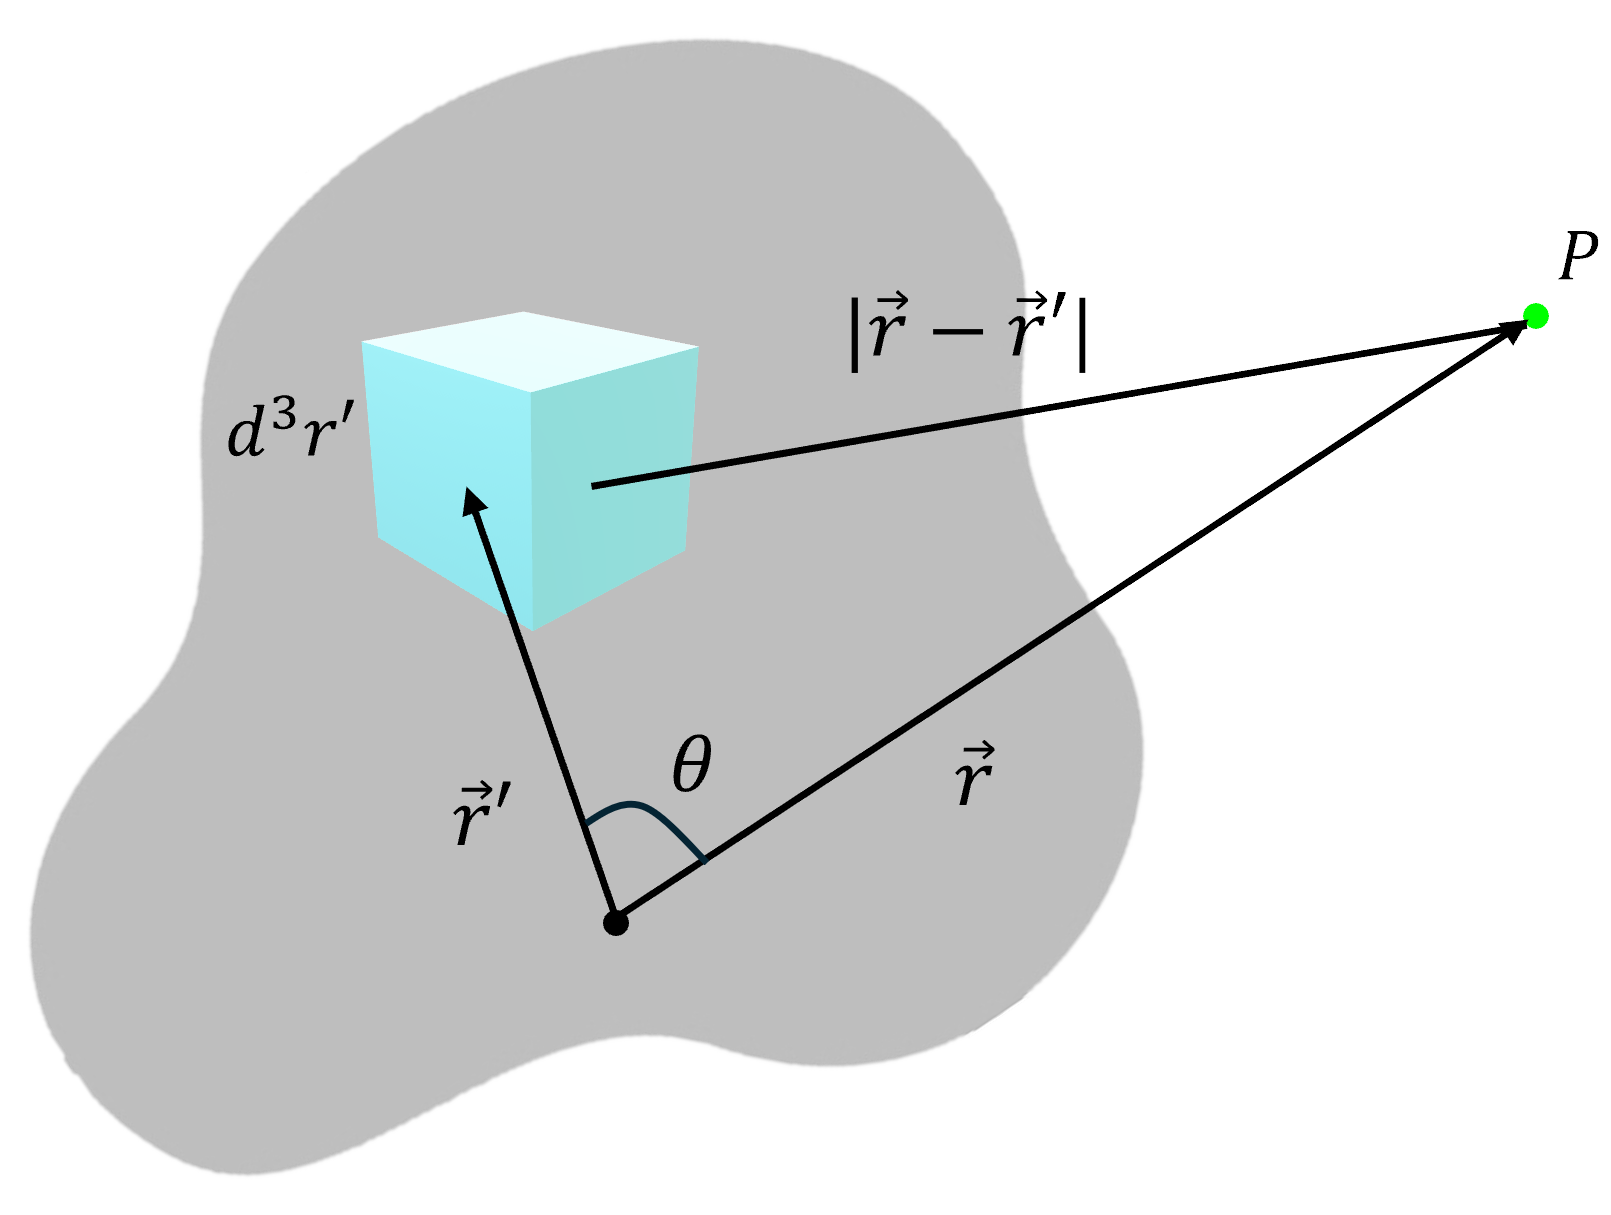
\includegraphics[width=6cm]{../../Figuras/aprox.png}
	\caption{Vector de posición $\Vec{r}\,'$ del elemento de volumen d$^3r'$ y vector de posición $\Vec{r}$. Se muestra el vector que apunta desde $\Vec{r}\,'$ a $\Vec{r}$,  $\Vec{r}-\Vec{r}\,'$ .}
	\label{vectposi}
\end{figure}
Al considerar únicamente el primer término de la expansión, se concluye que 
\begin{equation}
    \Vec{A}(\Vec{r})\approx\frac{\mu_0}{4\pi}\frac{e^{ikr}}{r}\int \Vec{J}(\Vec{r}\,') \text{d}^3r',    
    \label{aprox_pot_vec}
\end{equation}
que al realizar una integración por partes\footnote{Al considerar $\int_V \Vec{r}\,'[\nabla'\cdot\Vec{J}(\Vec{r}\,')]\text{d}^3r'=\int_{\partial V} \Vec{r}\,'[\Vec{J}(\Vec{r}\,')\cdot \text{d}\Vec{S}]\int_V \Vec{J}(\Vec{r}\,')\text{d}^3r'$ y asumiendo que $\Vec{J}$ se desvanece en los límites del volumen $V$, es decir, en la superficie $\partial V$. }, se obtiene que
\begin{equation}
	\int\Vec{J}(\vec{r}\,')d^3r'=-\int \Vec{r}\,'[\nabla'\cdot\Vec{J}(\vec{r}\,')]\text{d}^3r'=-i\omega\int \Vec{r}\,'\rho(\Vec{r}\,')\text{d}^3r',
	\label{Jrho}
\end{equation}
donde se empleó la ecuación de continuidad
\begin{equation*}
    \nabla\cdot\Vec{J}(\Vec{r}\,)=-\frac{\partial\rho(\Vec{r}\,)}{\partial t}=i\omega\rho(\Vec{r}\,). 
\end{equation*}
Al sustituir la Ec. (\ref{Jrho}) en la Ec. (\ref{aprox_pot_vec}) y considerando que el momento dipolar eléctrico $\Vec{p}$ de una distribución de cargas $\rho$ es
\begin{equation*}
	\Vec{p}=\int \Vec{r}\,'\rho(\Vec{r}\,')\text{d}^3r',
\end{equation*}
se obtiene \cite{Jackson}
\begin{equation}
    \Vec{A}(\Vec{r}\,)=-\frac{i\omega\mu_0}{4\pi}\frac{e^{ikr}}{r}\int \Vec{r}\,'\rho(\Vec{r}\,')\text{d}^3r'=-\frac{i\omega\mu_0}{4\pi}\frac{e^{ikr}}{r}\Vec{p}. 
    \label{A_dip}  
\end{equation}
Al emplear la ley de Faraday-Lenz para determinar el campo eléctrico y calcular el campo $\Vec{H}$ como el rotacional del potencial vectorial, se sigue que \cite{Jackson}
\begin{align}
	\Vec{E}&=\frac{1}{4\pi\epsilon_0}\left\{k^2(\hat{e}_r\times\Vec{p}\,)\times\hat{e}_r\frac{e^{ikr}}{r}+[3\hat{e}_r(\hat{e}_r\cdot\Vec{p}\,)-\Vec{p}\,]\left(\frac{1}{r^3}-\frac{ik}{r^2}\right)e^{ikr}\right\},\label{E}\\
    \Vec{H}&=\frac{ck^2}{4\pi}(\hat{e}_r\times\Vec{p}\,)\frac{e^{ikr}}{r}\left(1-\frac{1}{ikr}\right).    \label{H}
\end{align}
A partir de las Ecs. (\ref{E})  y (\ref{H}) se observa que el campo $\Vec{H}$ es transversal al vector radial en el campo lejano, mientras el campo eléctrico tiene componentes paralelas y perpendiculares a $\hat{e}_r$.\\ 

 De forma análoga al desarrollo de la Ec. (\ref{A_dip}) y empleando la Ley de Faraday-Lenz, en la zona de radiación cuando $kr\gg 1$, se tiene que al iluminar las cargas y corrientes en el sistema con una onda electromagnética de frecuencia angular $\omega$, se induce un dipolo eléctrico $\Vec{p}$ que genera campos electromagnéticos $\Vec{E}_p$ y $\Vec{H}_p$ y  que oscilan a la misma frecuencia $\omega$: 
\begin{align}
    \Vec{E}_p&=\frac{e^{ikr}}{-ikr}\frac{ik^3}{4\pi\epsilon_m}\hat{e}_r\times(\hat{e}_r\times \Vec{p}\,) e^{i\omega t}\qquad\text{y}\qquad
    \Vec{H}_p=\frac{ck^2}{4\pi}(\hat{e}_r\times\Vec{p}\,)\frac{e^{ikr}}{r}e^{i\omega t}.
\end{align}
En el caso particular en que la onda electromagnética incidente esté polarizada en la dirección $\hat{e}_x$, el momento dipolar inducido es $\Vec{p}=\epsilon_m \alpha E_0 e^{-i\omega t}\hat{e}_x$. Al reescribir al vector $\hat{e}_x$ en términos de la base de vectores esféricos como \cite{Griffiths}
\begin{equation}
	\hat{e}_x=\sin\theta\cos\phi\: \hat{e}_r+\cos\theta\cos\phi\: \hat{e}_{\theta}-\sin\phi \:\hat{e}_{\phi},
\end{equation}
se pueden reescribir a los campos generados por el dipolo inducido mediante el vector de amplitud de esparcimiento
\begin{equation}
	\Vec{X}=\frac{ik^3}{4\pi}\alpha \left[ \hat{e}_r\times(\hat{e}_r\times \hat{e}_x)\right]=\frac{ik^3}{4\pi}\alpha \left(-\cos\theta\cos\phi \hat{e}_{\theta}+\sin\phi \hat{e}_{\phi} \right),
	\label{Xvec}
\end{equation}
como \cite{Bohren}
 \begin{align}
 	\Vec{E}_{p}&=\frac{e^{ik(r-z)}}{-ikr}\Vec{X}\:E_0 e^{ikz}\qquad\text{y}\qquad
 	\Vec{H}_{p}=\frac{k}{\omega\mu}\hat{e}_r\times\Vec{E}_{p}.
 	\label{EH_s}
 \end{align}


\input{1Extinción,esp,abs}
\hypertarget{elipsoide}{\subsection{Elipsoide en la aproximación cuasiestática}}
Las secciones transversales de extinción, absorción y esparcimiento para distribuciones arbitrarias de cargas y corrientes confinadas a distancias cortas respecto al punto de observación fueron estudiadas en la sección anterior. En esta sección se estudia el caso particular del esparcimiento de luz por cargas y corrientes iluminadas por una onda plana electromagnética y confinadas en un elipsoide centrado en el origen, con semiejes $a,b,c$ alineados con los ejes $\uvec{x},\uvec{y},\uvec{z}$ respectivamente, y dimensiones tales que $\lambda\gg a>b>c$, a distancias alejadas del origen (ver Fig. \ref{elipse}), donde $\lambda$ es la longitud de onda que se relaciona con el vector de onda como $k=2\pi\sqrt{\epsilon_m/\lambda}$. A diferencia de la sección anterior, no se cuenta con simetría esférica, sin embargo es posible calcular una solución analítica, aproximada, al emplear las coordenadas elipsoidales confocales. \footnote{Existen diversas definiciones que pueden revisarse en \cite{ConfocalEllip}, sin embargo, se emplea la proporcionada en \cite{Arfken}. } Estas describen la superficie del elipsoide como \cite{ConfocalEllip}
\begin{equation}
	\frac{x^2}{a^2-u}+\frac{y^2}{b^2-u}+\frac{z^2}{c^2-u}=1,
	\label{elipsoide2}
\end{equation}
 donde debe determinarse el valor del parámetro $u$. La Ec. (\ref{elipsoide2}) es una ecuación de tercer grado para $u$, por lo que las soluciones (reales) son un conjunto de tres valores $\{\xi,\eta,\zeta\}$ tales que \footnote{La función $f(u)=x^2/(a^2-u)+y^2/(b^2-u)+z^2/(c^2-u)-1$ resulta ser continuamente diferenciable en el dominio $(-\infty, c^2)\cap (c^2, b^2)\cap (b^2, a^2)$ y estrictamente creciente en cada intervalo que lo compone, de tal forma que, al calcular los límites en cada extremo de los intervalos, se concluye que existe exactamente una raíz en cada intervalo.}
\begin{equation}
	-\infty<\xi<c^2<\eta<b^2<\zeta<a^2
\end{equation}
que corresponden a tres formas cuádricas con focos en común (ver Fig. \ref{Quadrics}). Estas se relacionan con las coordenadas cartesianas mediante el siguiente sistema de ecuaciones escrito en forma matricial
\begin{center}
	\resizebox{0.44\textwidth}{!}{
	\begin{equation*}
		\begin{pmatrix}
			\frac{1}{a^2+\xi} & \frac{1}{b^2+\xi} & \frac{1}{c^2+\xi}\\
			\frac{1}{a^2+\eta} & \frac{1}{a^2+\eta} & \frac{1}{a^2+\eta}\\
			\frac{1}{a^2+\zeta} & \frac{1}{a^2+\zeta} & \frac{1}{a^2+\zeta}\end{pmatrix}\begin{pmatrix}
			x^2\\
			y^2\\
			z^2
		\end{pmatrix}=\begin{pmatrix}
			1\\
			1\\
			1\\
		\end{pmatrix},
	\end{equation*}
}
\end{center}
cuya solución está dada por las expresiones
\begin{align}
	x^2&=\frac{(a^2+\xi)(a^2+\eta)(a^2+\zeta)}{(b^2-a^2)(c^2-a^2)},\label{x_elips}\\
	y^2&=\frac{(b^2+\xi)(b^2+\eta)(b^2+\zeta)}{(a^2-b^2)(c^2-b^2)},\label{y_elips}\\
	z^2&=\frac{(c^2+\xi)(c^2+\eta)(c^2+\zeta)}{(a^2-c^2)(b^2-c^2)}. \label{z_elips}    
\end{align}
A partir del sistema de ecuaciones anterior, se puede observar que cuando $\xi$ es constante, se obtiene un elipsoide. De esta forma, la superficie de la partícula a estudiar se tiene cuando $\xi=0$. Mientras que si $\eta$ es constante, se obtiene un hiperboloide de una hoja y cuando $\zeta$ es constante se tiene un hiperboloide de dos hojas. Cada punto ($x,y,z$) tiene una correspondencia única con ($\xi,\eta,\zeta$), pero la transformación inversa no es biyectiva, ya que cada ($\xi,\eta,\zeta$) se asocia a ocho puntos simétricos respecto a los ejes ($x,y,z$). \cite{Cambdrige} \\

\begin{figure}[H]
	\centering
	\sidesubfloat[][a]{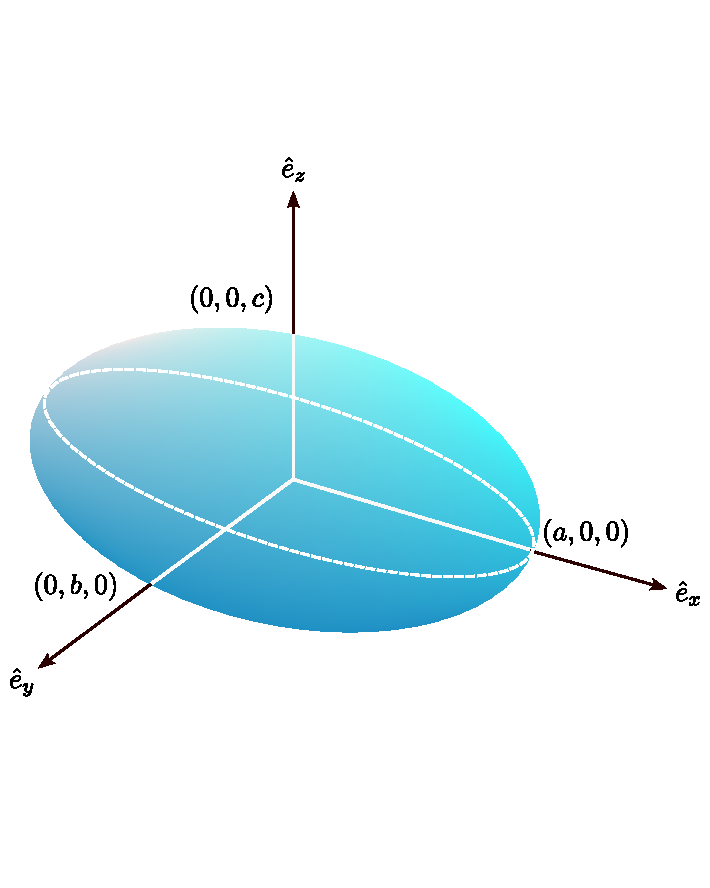
\includegraphics[width=0.45\textwidth]{../../Figuras/ellipsoid}\label{elipse}}
	\sidesubfloat[][b]{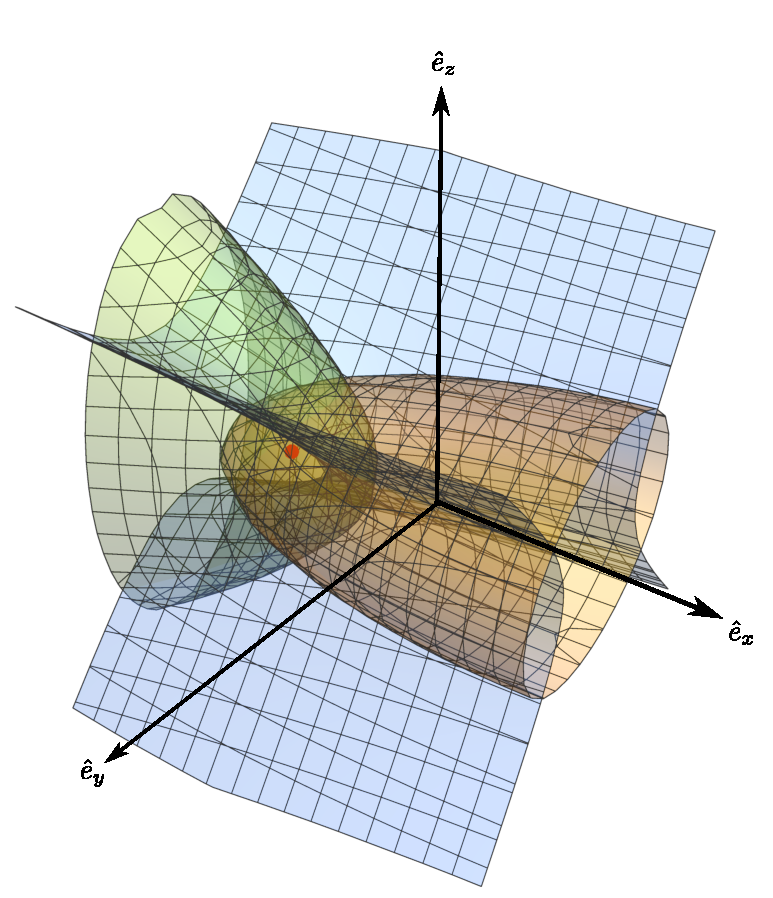
\includegraphics[width=0.45\textwidth]{../../Figuras/quadraticonfo}\label{Quadrics}}
	\caption{Sistema a estudiar. \textbf{a)} Elipsoide centrado en el origen, con semiejes $a, b, c$ tales que $a > b > c.$   \textbf{b)} Superficies confocales. Hiperboloide de una hoja (superficie azul) con $u=0.8$, hiperboloide de dos hojas (superficie verde) con $u=0.5$ y elipsoide (superficie naranja) con $u=0.1$. Todas las superficies poseen semiejes con valores $a=1, b=0.8$ y $c=0.6$. El punto rojo representa uno de los focos en común localizado en (-0.8,0,0).}
	\label{ConfocalQuadrics}
\end{figure}



En el problema de esparcimento de luz sin retardo (o límite cuasiestático) se resuelve la ecuación de Laplace para el potencial eléctrico. En un sistema coordenado general, esta ecuación se escribe en términos de coordenadas generalizadas \cite{Arfken}
\begin{equation}
	\nabla^2\phi=\frac{1}{h_1h_2h_3}\left[\frac{\partial}{\partial q_1}\left(\frac{h_2h_3}{h_1}\frac{\partial\phi}{\partial q_1}\right)+\frac{\partial}{\partial q_2}\left(\frac{h_3h_1}{h_2}\frac{\partial\phi}{\partial q_2}\right)+\frac{\partial}{\partial q_3}\left(\frac{h_1h_2}{h_3}\frac{\partial\phi}{\partial q_3}\right)\right],
	\label{laplaciano}    
\end{equation}
donde $\phi$ es una función escalar, y  $h_i$ con $i=1,2,3$ los factores de escala que, para coordenadas elipsoidales se asocian como $1\rightarrow\xi, 2\rightarrow\eta$ y $3\rightarrow\zeta,$ y se determinan al hacer un cambio de base de coordenadas cartesianas a elipsoidales. Estos factores de escala están dados por \cite{Arfken}
\begin{equation}
	h_i=\Big|\frac{\partial \Vec{r}}{\partial q_i}\Big|=\sqrt{\left(\frac{\partial x}{\partial q_i}\right)^2+\left(\frac{\partial y}{\partial q_i}\right)^2+\left(\frac{\partial z}{\partial q_i}\right)^2}.
\end{equation} 
Que para coordenadas elipsoidales, considerando la variación en la dirección $x$, empleando la Ec. (\ref{x_elips}), se tiene que \begin{align*}
	\frac{\partial x}{\partial \xi}&=\frac{1}{2}\left(\frac{(a^2+\xi)(a^2+\eta)(a^2+\zeta)}{(b^2-a^2)(c^2-a^2)}\right)^{-1/2}\frac{\partial}{\partial \xi}\left(\frac{(a^2+\xi)(a^2+\eta)(a^2+\zeta)}{(b^2-a^2)(c^2-a^2)}\right)\nonumber\\
	&=\frac{1}{2}\frac{1}{a^2+\xi}\sqrt{\frac{(a^2+\xi)(a^2+\eta)(a^2+\zeta)}{(b^2-a^2)(c^2-a^2)}}\nonumber\\
	&=\frac{1}{2x}\frac{\partial x^2}{\partial\xi},
\end{align*}
por tanto,
\begin{equation*}
	\frac{\partial x}{\partial \xi}=\frac{1}{2}\frac{x}{(a^2+\xi)}.
\end{equation*}
Empleando las Ecs. (\ref{y_elips}) y (\ref{z_elips}) para $y$ y $z$, respectivamente, se obtiene
\begin{align*}
	\frac{\partial y}{\partial \xi}&=\frac{1}{2y}\frac{\partial y^2}{\partial\xi}=\frac{1}{2}\frac{y}{(b^2+\xi)},\\
	\frac{\partial z}{\partial \xi}&=\frac{1}{2z}\frac{\partial z^2}{\partial\xi}=\frac{1}{2}\frac{z}{(c^2+\xi)}.
\end{align*}
De esta forma, el cuadrado del primer factor de escala $h_1$ es
\begin{equation}
	h_1^2=\frac{1}{4}\left[\frac{x^2}{(a^2+\xi)^2}+\frac{y}{(b^2+\xi)^2}+\frac{z}{(c^2+\xi)^2}\right];
	\label{h1}
\end{equation}
y por economía, se define a la función $g(u)=(u-\xi)(u-\eta)(u-\zeta)$, que permite reescribir la Ec. (\ref{elipsoide2}) como
\begin{equation}
	1-\frac{x^2}{a^2+u}-\frac{y^2}{b^2+u}-\frac{z^2}{c^2+u}=\frac{g(u)}{(a^2+u)(b^2+u)(c^2+u)},
\end{equation}
donde $g(u)$ es una función cúbica con tres raíces reales dentro del rango descrito por las limitaciones de cada variable, y al  derivarla con respecto de $u$ se obtiene
\begin{align}
	\frac{x^2}{(a^2+u)^2}+\frac{y^2}{(b^2+u)^2}+\frac{z^2}{(c^2+u)^2}&=\frac{g(u)}{[f(u)]^2}\left[\frac{1}{u-\xi}+\frac{1}{u-\zeta}+\frac{1}{u-\eta}-\left(\frac{1}{a^2+u}+\frac{1}{b^2+u}+\frac{1}{c^2+u}\right)\right],
\end{align}
con 
\begin{equation}
	f(u)=\sqrt{(a^2+u)(b^2+u)(c^2+u)},  
\end{equation}
por medio del cual se puede reescribir al primer factor de escala de la Ec. (\ref{h1}) como
\begin{align*}
	h_1^2&=\frac{1}{4}\frac{g(u)}{[f(u)]^2}\left[\frac{(u-\zeta)(u-\eta)+(u-\xi)(u-\eta)+(u-\xi)(u-\zeta)}{g(u)}-\left(\frac{1}{a^2+u}+\frac{1}{b^2+u}+\frac{1}{c^2+u}\right)\right].    
\end{align*}
Dado que $\xi$ es una raíz de $g(u)$, entonces, $g(u)=0$, por lo que el factor de escala $h_1$ es
\begin{equation}
	h_1=\frac{\sqrt{(\xi-\eta)(\xi-\zeta)}}{2f(\xi)}.
	\label{h1}
\end{equation}
Mediante un proceso semejante, se tiene que \cite{Arfken}
\begin{equation}
	h_2=\frac{\sqrt{(\eta-\xi)(\eta-\zeta)}}{2f(\eta)}\hspace{0.5cm}\mbox{y}\hspace{0.5cm}
	h_3=\frac{\sqrt{(\zeta-\xi)(\zeta-\eta)}}{2f(\zeta)}.
	\label{h2yh3}
\end{equation}
Sustituyendo las Ecs. (\ref{h1}) y (\ref{h2yh3}) en la Ec. (\ref{laplaciano}) y simplificando,
\begin{align*}
	\nabla^2\phi=\frac{4}{\Upsilon}\left[(\eta-\zeta)f(\xi)\frac{\partial}{\partial\xi}\left(f(\xi)\frac{\partial\phi}{\partial\xi}\right)+(\zeta-\xi)f(\eta)\frac{\partial}{\partial\eta}\left(f(\eta)\frac{\partial\eta}{\partial\eta}\right)+(\xi-\zeta)f(\zeta)\frac{\partial}{\partial\zeta}\left(f(\zeta)\frac{\partial\phi}{\partial\zeta}\right)\right],
\end{align*}
donde a $\Upsilon$ se le conoce como el valor absoluto del determinante funcional \cite{Kellog}
\begin{equation}
	\Upsilon=(\xi-\eta)(\zeta-\xi)(\eta-\zeta).
\end{equation}
Como resultado de lo anterior, la ecuación de Laplace en coordenadas elipsoidales se reescribe como
\begin{equation}
	\nabla^2\phi=(\eta-\zeta)f(\xi)\frac{\partial}{\partial\xi}\left(f(\xi)\frac{\partial\phi}{\partial\xi}\right)+(\zeta-\xi)f(\eta)\frac{\partial}{\partial\eta}\left(f(\eta)\frac{\partial\eta}{\partial\eta}\right)+(\xi-\eta)f(\zeta)\frac{\partial}{\partial\zeta}\left(f(\zeta)\frac{\partial\phi}{\partial\zeta}\right)=0.
	\label{laplaceplisoidal}
\end{equation}
Una de las formas por la cual se puede resolver la ecuación anterior es mediante el método de reducción de orden, el cual proporciona una solución linealmente independiente a partir de otra conocida con anterioridad \cite{Braun}. En este contexto, $\phi$ corresponde a la solución de dicha ecuación que está determinada por la forma del campo incidente y cumple las condiciones de frontera. \\


El potencial eléctrico solución a la Ec. (\ref{laplaceplisoidal}) hereda la simetría del sistema de interés, el cual consiste en un elipsoide homogéneo iluminado por un campo eléctrico incidente uniforme alineado a lo largo del eje $\uvec{z}$. Por tanto,  a cada punto del espacio descrito por las coordenadas elipsoidales le corresponden ocho puntos en las coordenadas cartesianas. Es decir, las propiedades de simetría del sistema en el potencial eléctrico son:
\begin{equation}
    \phi(x,y,z)=\phi(-x,y,z)=\phi(x,-y,z)=\phi(-x,-y,z),
\end{equation}
\begin{equation}
    \phi(x,y,-z)=\phi(-x,y ,-z)=\phi(x,-y,-z)=\phi(-x,-y,-z),
\end{equation}
donde $z$ es positiva. Entonces, solo se tiene que considerar el potencial en dos octantes: uno con $z$ positivo y otro con $z$ negativo. \\

Dado que se quiere determinar el potencial eléctrico producido de la interacción entre el campo eléctrico externo y la distribución de cargas y corrientes confinadas en un elipsoide, se propone dividir el problema en dos regiones espaciales: al exterior y al interior del elipsoide, de modo que el potencial total se puede expresar como la contribución del potencial en el exterior del elipsoide $\phi_{ext}$  y la contribución en el interior de este $\phi_{int}$. Asimismo, se propone descomponer al potencial $\phi_{ext}$ en una contribución de la onda plana incidente $\phi_0$ y en otra de perturbación $\phi_p$, la cual correspondería al campo eléctrico esparcido por la partícula
\begin{equation}
	\phi_{ext}(\xi,\eta,\zeta)=\phi_0(\xi,\eta,\zeta)+\phi_p(\xi,\eta,\zeta),    
\end{equation}
donde, de acuerdo con la expresión para $z$ en la Ec. (\ref{z_elips}),
\begin{equation}
	\phi_0=-E_0 r\cos\theta=-E_0 z=-E_0\left[\frac{(c^2+\xi)(c^2+\eta)(c^2+\zeta)}{(a^2-c^2)(b^2-c^2)}\right]^{1/2}.
	\label{pot_0}
\end{equation}

Al considerar las condiciones de frontera en el sistema en dos límites: a distancias muy lejanas del elipsoide y en la interfaz entre el medio y el elipsoide, debido al teorema de unicidad \cite{Griffiths}, el problema queda totalmente determinado. Para distancias lo suficientemente lejanas a la partícula, es decir, cuando $\xi\gg a^2$, al factorizar $\xi$ de  la Ec. (\ref{x_elips}), se obtiene
\begin{equation*}
    \frac{x^2}{a^2/\xi+1}+\frac{y^2}{b^2/\xi+1}+\frac{z^2}{c^2/\xi+1}=\xi,
\end{equation*}
donde
\begin{equation*}
    \lim_{\xi\rightarrow\infty}\left(\frac{x^2}{a^2/\xi+1}+\frac{y^2}{b^2/\xi+1}+\frac{z^2}{c^2/\xi+1}\right)=x^2+y^2+z^2=r^2,
\end{equation*}
entonces, $\xi \simeq r^2$ en el límite asintótico. Asimismo, en esta aproximación el potencial de perturbación es despreciable, por lo que 
\begin{equation}
\lim_{\xi\rightarrow\infty}\phi_p=0
\label{limitephi_p}.
\end{equation}
Al considerar $\phi_{int}$ y $\epsilon_p$ el potencial y la permitividad eléctrica en el interior del elipsoide y las mismas cantidades $\phi_{ext}$ y $\epsilon_m$ para el exterior de este, como el potencial es continuo en la superficie del elipsoide y la componente perpendicular a la superficie del elipsoide del campo de desplazamiento eléctrico $\Vec{D}$ por ausencia de cargas externas también \cite{Griffiths}
\begin{subequations}
\label{condicionesfrontera}
\begin{align}
    \phi_{int}|_{\xi=0}&=\phi_{ext}|_{\xi=0}\label{cf1},\\
    \epsilon_p\frac{\partial \phi_{int}}{\partial \xi}\Big |_{\xi=0}&=
    \epsilon_m\frac{\partial \phi_{ext}}{\partial \xi}\Big |_{\xi=0}\label{cf2},
\end{align}
\end{subequations}
en donde se emplea la relación constitutiva $\Vec{D}=\epsilon\Vec{E}$ y que $E_{int}^{\perp}=-\partial \phi_{int} /\partial \xi$.\\


Reescribiendo los potenciales $\phi_{int}$ y $\phi_0$ de la forma
\begin{align}
    \phi(\xi,\eta,\zeta)&=F(\xi)[(c^2+\eta)(c^2+\zeta)]^{1/2}, 
    \label{phi0 con F}
\end{align}
se obtiene que, para que satisfagan la Ec. (\ref{laplaceplisoidal}), se tiene que cumplir 
\begin{equation}
  (\eta-\zeta)[(c^2+\zeta)(c^2+\eta)]^{1/2}\left[f(\xi)\frac{\text{d}}{\text{d}\xi}\left(f(\xi)\frac{ \text{d} F(\xi)}{\text{d}\xi}\right)-\frac{1}{4}F(\xi)(a^2+b^2+2\xi)\right]=0,
\end{equation}
lo cual es equivalente a resolver
\begin{equation}
    f(\xi)\frac{\text{d}}{\text{d}\xi}\left(f(\xi)\frac{ \text{d} F(\xi)}{\text{d}\xi}\right)-\left(\frac{a^2+b^2}{4}+\frac{\xi}{2}\right)F(\xi)=0.
    \label{ecsimpli}
\end{equation}
La ecuación anterior es una ecuación diferencial ordinaria lineal de segundo orden, con dos soluciones no triviales linealmente independientes. Una de estas soluciones es
\begin{equation}
    F_1(\xi)=(c^2+\xi)^{1/2},
    \label{F1}
\end{equation}
y la segunda solución se obtiene mediante el método de reducción de orden. Como $F_1(\xi)$ es solución de la Ec. (\ref{laplaceplisoidal}), se propone una segunda solución dada por $F_2(\xi)=v(\xi)F_1(\xi)$ donde $v(\xi)$ se determina al sustituir dicha solución en la ecuación diferencial dada, reduciéndola a una ecuación de primer orden donde la variable dependiente será $v$. Derivando la ecuación anterior respecto a $\xi$
\begin{align*}
    \frac{\text{d}F_2(\xi)}{\text{d}\xi}&=F_1(\xi)\frac{\text{d}v(\xi)}{\text{d}\xi}+v(\xi)\frac{F_1(\xi)}{\text{d}\xi},\\
    \frac{\text{d}^2F_2(\xi)}{\text{d}\xi^2}&=F_1(\xi)\frac{\text{d}^2v(\xi)}{\text{d}\xi^2}+2\frac{\text{d}v(\xi)}{\text{d}\xi}\frac{\text{d}F_1(\xi)}{\text{d}\xi}+v(\xi)\frac{\text{d}^2F_1(\xi)}{\text{d}\xi^2},
\end{align*}
y sustituyendo las derivadas anteriores en la Ec. (\ref{F1}) y simplificando, se obtiene
\begin{equation*}
    f^2(\xi)F_1(\xi)\frac{\text{d}^2v(\xi)}{\text{d}\xi^2}+\frac{\text{d}v(\xi)}{\text{d}\xi}\left[f(\xi)F_1(\xi)\frac{\text{d}f(\xi)}{\text{d}\xi}+2f^2(\xi)\frac{\text{d}F_1(\xi)}{\text{d}\xi}\right]=0.
\end{equation*}
Haciendo el cambio de variable $V(\xi)=dv(\xi)/d\xi$ y reordenando términos resulta en
\begin{equation*}
    \frac{1}{V(\xi)}\frac{\text{d}V(\xi)}{\text{d}\xi}=-\frac{1}{f^2(\xi)F_1(\xi)}\left[f(\xi)F_1(\xi)\frac{\text{d}f(\xi)}{\text{d}\xi}+2f^2(\xi)\frac{\text{d}F_1(\xi)}{\text{d}\xi}\right],
\end{equation*}
donde la integral indefinida de la ecuación anterior da como resultado
\begin{align*}
    \ln[V(q)]=-\ln[F_1^2(q)f(q)],
\end{align*}
entonces,
\begin{equation*}
    \frac{\text{d}v(q)}{\text{d}q}=\frac{1}{F_1^2(q)f(q)}.
\end{equation*}
Como $\text{d}v(q)/\text{d}q$ es distinto de cero,  $v(q)$ es distinto de una constante. Integrando lo anterior se tiene que
\begin{equation*}
    v(\xi)=\int_{\xi}^{\infty}\frac{\text{d}q}{F_1^2(q)f(q)},
\end{equation*}
por lo tanto, 
\begin{equation}
  F_2(\xi)=F_1(\xi)\int_{\xi}^{\infty}\frac{\text{d}q}{F_1^2(q)f(q)}.
  \label{F2}
\end{equation}
Al escribir explícitamente el integrando, usando las Ecs. (\ref{F1}) y (\ref{F2}), y haciendo una integración por partes con $u=1/(a^2+q)^{1/2}$ y $\text{d}v=1/[(c^2+q)^{3/2}(b^2+q)^{1/2}]$ se obtiene
\begin{align}
    F_2(\xi)&=F_1(\xi)\int_{\xi}^{\infty}\frac{\text{d}q}{(c^2+q)[(a^2+q)(b^2+q)(c^2+q)]^{1/2}}\nonumber\\
    &=\frac{F_1(\xi)}{c^2-b^2}\left[\frac{b^2+q}{(a^2+q)(c^2+q)}\right]^{1/2}\Bigg|_\xi^{\infty}-\int_\xi^{\infty}\sqrt{\frac{b^2+q}{c^2+q}}\frac{\text{d}q}{(c^2-b^2)(a^2+q)^{3/2}}.
\end{align}
Reescribiendo la segunda integral
\begin{equation}
	\int_\xi^{\infty}\frac{\sqrt{\frac{b^2+q}{a^2+q}}\sqrt{\frac{b^2+q}{a^2+q}}\sqrt{a^2-c^2}\:\text{d}q}{\sqrt{a^2-c^2}(c^2-b^2)\sqrt{\frac{c^2+q}{a^2+q}}\sqrt{\frac{b^2+q}{c^2+q}}(a^2+q)^{3/2}\sqrt{\frac{c^2+q}{a^2+q}}},\label{eliptic}
\end{equation}
y considerando que
\begin{equation*}
	\frac{\text{d}}{\text{d}q}\left(E\left(\mbox{arcsen}\left(\frac{\sqrt{a^2-c^2}}{\sqrt{a^2+q}}\right)\Bigg|\frac{a^2-b^2}{a^2-c^2}\right)\right)=-\frac{\sqrt{\frac{b^2+q}{a^2+q}}\sqrt{a^2-c^2}}{(a^2+q)^{3/2}\sqrt{\frac{c^2+q}{a^2+q}}}
\end{equation*}
al sustituir en la Ec. (\ref{eliptic}) y haciendo uso del teorema fundamental del cálculo, se obtiene que la segunda solución a la Ec. (\ref{ecsimpli}) es 
\begin{align}
    F_2(\xi)&=\frac{2F_1(\xi)}{c^2-b^2}\Bigg\{\left[\frac{b^2+q}{(a^2+q)(c^2+q)}\right]^{1/2}-\frac{1}{(a^2-c^2)^{1/2}}E\left(\mbox{arcsen}\left(\frac{\sqrt{a^2-c^2}}{a^2+q}\right)\Bigg|\frac{a^2-b^2}{a^2-c^2}\right)\Bigg\}\Bigg|_\xi^{\infty},
\end{align}
donde $E(\phi|m)$ es una integral elíptica de segundo tipo definida como \cite{Abramowitz}
\begin{equation}
    E(x|\kappa)=\int_{0}^x\frac{\sqrt{1-\kappa^2t^2}}{1-t^2}\text{d}t,\hspace{1cm}0\leq m\leq 1,
\end{equation}
donde el módulo angular es $\beta=\mbox{arcsen}\:\kappa$ y $\kappa$ es la excentricidad. En el primer límite de integración ($\infty$) de $F_2(\xi)$ al evaluar se obtiene que el primer sumando es cero, y en el segundo límite la función arcoseno es cero. De esta forma, la parte angular de la integral es cero, es decir, $E(0|m)=0$. En consecuencia, considerando la definición de $F_1$ en la Ec. (\ref{F1}) se tiene que $F_1$ y $F_2$ cumplen

\begin{equation}
    \lim_{\xi \to 0}F_1(\xi)=c\hspace{1cm}\mbox{y}\hspace{1cm} \lim_{\xi \to \infty}F_2(\xi)=0.
\end{equation}
De esta forma, considerando que $F_1$ no satisface la condición impuesta sobre $\phi_p$ en la Ec. (\ref{limitephi_p}) y que necesariamente el potencial dentro de la partícula debe de ser finito, lo cual $F_2$ no satisface, los potenciales $\phi_{int}$ y $\phi_p$, propuestos como en la Ec. (\ref{phi0 con F}), están dados por
\begin{align}
    \phi_{int}&=C_1F_1(\xi)[(c^2+\eta)(c^2+\zeta)]^{1/2}\label{phi_int},\\
    \phi_p&=C_2F_2(\xi)[(c^2+\eta)(c^2+\zeta)]^{1/2}\label{phi_p},
\end{align}
donde $C_1$ y $C_2$ son constantes a determinar a partir de las condiciones de frontera dadas por las Ecs. (\ref{condicionesfrontera}). Empleando la primera condición de contorno [Ec. (\ref{cf1})]
\begin{equation*}
    C_1F_1(\xi)[(c^2+\eta)(c^2+\zeta)]^{1/2}=E_0\left[\frac{(c^2+\xi)(c^2+\eta)(c^2+\zeta)}{(a^2-c^2)(b^2-c^2)}\right]^{1/2}+C_2F_2(\xi)[(c^2+\eta)(c^2+\zeta)]^{1/2},
\end{equation*}
y al sustituir las Ecs. (\ref{F1}) y (\ref{F2}) en la ecuación anterior se obtiene
\begin{align}
    C_2 \int_{0}^{\infty}\frac{\text{d}q}{(c^2+q)f(q)}-C_1&=\frac{E_0}{[(a^2-c^2)(b^2-c^2)]^{1/2}}.
    \label{C2}
\end{align}
Al definir
\begin{equation}
    L^{(3)}=\frac{abc}{2}\int_{0}^{\infty}\frac{\text{d}q}{(c^2+q)f(q)},
\end{equation}
entonces, se puede reescribir la Ec. (\ref{C2}) como
\begin{equation}
    C_2L^{(3)}\left(\frac{2}{abc}\right)-C_1=\frac{E_0}{[(a^2-c^2)(b^2-c^2)]^{1/2}},
    \label{ec1 de cf}
\end{equation}
y, al usar la segunda condición de contorno [Ec. (\ref{cf2})], se obtiene
\begin{align*}
    \frac{\epsilon_pC_1}{2}\left[\frac{(c^2+\eta)(c^2+\zeta)}{(c^2+\xi)}\right]^{1/2}&=\frac{\epsilon_mE_0}{2}\left[\frac{(c^2+\eta)(c^2+\zeta)}{(c^2+\xi)(a^2-c^2)(b^2-c^2)}\right]^{1/2}+\frac{\epsilon_m C_2}{2}\left[\frac{(c^2+\eta)(c^2+\zeta)}{(c^2+\xi)}\right]^{1/2}\int_{\xi}^{\infty}\frac{\text{d}q}{(c^2+q)f(q)}\\
   &+\epsilon_mC_2[(c^2+\xi)(c^2+\eta)(c^2+\zeta)]^{1/2}\frac{\text{d}}{\text{d}\xi}\Bigg\{\int_{\xi}^{\infty}\frac{\text{d}q}{(c^2+q)f(q)}\Bigg\},
\end{align*}
donde la integral del tercer sumando es
\begin{align*}
    \frac{\text{d}}{\text{d}\xi}\left[\int_{\xi}^{\infty}\frac{\text{d}q}{(c^2+q)f(q)}\right]&=\frac{\text{d}}{\text{d}\xi}\left[\lim_{a\to\infty}\int_{\xi}^{a}\frac{\text{d}q}{(c^2+q)f(q)}\right]=-\lim_{a\to\infty}\frac{1}{(c^2+\xi)f(\xi)}=-\frac{1}{(c^2+\xi)f(\xi)};
\end{align*}
de tal forma que, al evaluar en $\xi=0$, se obtiene
\begin{equation}
    \epsilon_m C_2\left(\frac{2}{abc}\right)\left(L^{(3)}-1\right)- \epsilon_p C_1=\frac{\epsilon_m E_0}{[(a^2-c^2)(b^2-c^2)]^{1/2}}.
     \label{ec2 de cf}
\end{equation}
Las constantes $C_1$ y $C_2$ se obtienen a partir de  resolver el sistema de ecuaciones entre las Ecs. (\ref{ec1 de cf}) y (\ref{ec2 de cf}), al multiplicar la Ec. (\ref{ec1 de cf}) por $\epsilon_p$ y restarle la Ec. (\ref{ec2 de cf}), al simplificar se obtiene que
\begin{equation*}
    C_2=\frac{abc}{2}\frac{E_0(\epsilon_p-\epsilon_m)}{[(a^2-c^2)(b^2-c^2)]^{1/2}}\left[L^{(3)}(\epsilon_p-\epsilon_m)+\epsilon_m\right]^{-1},
\end{equation*}
por lo tanto, al sustituir $C_2$ en la Ec. (\ref{ec1 de cf}) se obtiene una expresión para $C_1$
\begin{equation*}
    C_1=\frac{E_0}{[(a^2-c^2)(b^2-c^2)]^{1/2}}\Bigg\{ \left[1+\frac{\epsilon_m}{L^{(3)}(\epsilon_p-\epsilon_m)}\right]^{-1}-1\Bigg\}.
\end{equation*}
De esta forma, ya se puede determinar el potencial dentro de la partícula sustituyendo $F_1$ y $C_1$ en la Ec. (\ref{phi_int}), por lo que
\begin{equation}
	\phi_{int}=\frac{1}{1+\dfrac{L^{(3)}(\epsilon_p-\epsilon_m)}{\epsilon_m}}\phi_0,
\end{equation}

\begin{equation}
	\phi_p=\frac{abc}{2}\frac{\dfrac{(\epsilon_m-\epsilon_p)}{\epsilon_m}{\displaystyle\int_{\xi}^{\infty}}\dfrac{\text{d}q}{F_1^2(q)f(q)}}{1+\dfrac{L^{(3)}(\epsilon_p-\epsilon_m)}{\epsilon_m}}\phi_0.
\end{equation}
A pesar de que inicialmente se había considerado el octante donde $x,y,z$ eran positivas, las ecuaciones anteriormente obtenidas representan el potencial en todos los puntos del espacio, como consecuencia de la simetría de la partícula.\\

Al considerar distancias $r$ muy alejadas del origen tales que $\xi\simeq r^2\gg a^2$
\begin{equation*}
    \int_{\xi}^{\infty}\frac{\text{d}q}{F_1^2(q)f(q)}= \int_{\xi}^{\infty}\frac{\text{d}q}{(c^2+q)f(q)}=\int_{\xi}^{\infty}\frac{\text{d}q}{q^{5/2}}=\frac{2}{3}\xi^{-3/2},
\end{equation*}
y entonces el potencial $\phi_p$ está dado por
\begin{equation}
    \phi_p\sim\left(\dfrac{E_0\cos\theta}{r^2}\right)\dfrac{\left(\dfrac{abc}{3}\right)\left(\dfrac{\epsilon_p-\epsilon_m}{\epsilon_m}\right)}{1+\dfrac{L^{(3)}(\epsilon_p-\epsilon_m)}{\epsilon_m}},\hspace{1cm}(r\gg a)
\end{equation}
cuya expresión es equivalente a la de un dipolo puntual dado por
\begin{equation}
    \Vec{p}=4\pi\epsilon_m abc\frac{\epsilon_p-\epsilon_m}{3\epsilon_m+3L^{(3)}(\epsilon_p-\epsilon_m)}\Vec{E}_0
    \label{momento_dip}.
\end{equation}
Entonces, la polarizabilidad $\alpha^{(3)}$ de un elipsoide en un campo paralelo al eje $z$ es
\begin{equation}
    \alpha^{(3)}=V\frac{\epsilon_p-\epsilon_m}{\epsilon_m+L^{(3)}(\epsilon_p-\epsilon_m)},
\end{equation}
donde $V=4\pi abc/3$ es el volumen del elipsoide. De manera análoga, las polarizabilidades $ \alpha^{(1)}$ y $ \alpha^{(2)}$ cuando el campo es aplicado en los ejes $\hat{e}_x$ y $\hat{e}_y$ son
\begin{align*}
    \alpha^{(1)}&=4\pi abc \frac{\epsilon_p-\epsilon_m}{3\epsilon_m+3L^{(1)}(\epsilon_p-\epsilon_m)},&
    \alpha^{(2)}&=4\pi abc \frac{\epsilon_p-\epsilon_m}{3\epsilon_m+3L^{(2)}(\epsilon_p-\epsilon_m)},
\end{align*}
donde 
\begin{align*}
    L^{(1)}&=\frac{abc}{2}\int_{0}^{\infty}\frac{\text{d}q}{(a^2+q)f(q)},&\text{y} && 
    L^{(2)}&=\frac{abc}{2}\int_{0}^{\infty}\frac{\text{d}q}{(b^2+q)f(q)}.
\end{align*}
Se puede concluir en general que la polarizabilidad en una dirección arbitraria $j$, paralela a algún eje cartesiano es
\begin{equation}
    \alpha^{(j)}=V\frac{\epsilon_p-\epsilon_m}{\epsilon_m+L^{(j)}(\epsilon_p-\epsilon_m)}
\end{equation}
con $L^{(j)}$ conocido como \textit{factor geométrico}, dado por la integral 
\begin{equation}
    L^{(j)}=\frac{abc}{2}\int_0^{\infty}\frac{\text{d}q}{(a_j^2+q)f(q)}
\end{equation}
donde el superíndice ($j$) indica la dirección en la que se calcula el factor de geométrico y $a_j$ denota al semieje del elipsoide orientado en esa misma dirección. Cabe mencionar que los factores geométricos  satisfacen que, por definición, $L^{(1)}\leq L^{(2)}\leq L^{(3)}$, y que sólo dos de los tres son independientes, ya que tienen que cumplir la relación 
\begin{equation}
    L^{(1)}+L^{(2)}+L^{(3)}=1,
    \label{rel_fac_geom}
\end{equation}
pues, 
\begin{equation*}
	L^{(1)}+L^{(2)}+L^{(3)}=\frac{abc}{2}\int_0^{\infty}\left[\frac{1}{(a^2+q)}+\frac{1}{(b^2+q)}+\frac{1}{(c^2+q)}\right]\frac{\text{d}q}{f(q)},
\end{equation*}
que al simplificar se obtiene
$$L^{(1)}+L^{(2)}+L^{(3)}=-abc\int_0^{\infty}\frac{\text{d}}{\text{d}q}\left(\frac{1}{f(q)}\right)\text{d}q,$$
que puede resolverse de forma analítica mediante el teorema fundamental del cálculo. Este procedimiento deviene en
\begin{align*}
	\int_0^{\infty}\frac{\text{d}}{\text{d}q}\left(\frac{1}{f(q)}\right)\text{d}q=\frac{1}{f(q)}\Big|_{(abc)^2}^{\infty}=-\frac{1}{abc},
\end{align*}
y por consiguiente, se cumple la Ec. (\ref{rel_fac_geom}).\\

\noindent En el caso en el que los semiejes son iguales ($a=b=c$), es decir, en el caso de una esfera se tiene que
\begin{equation*}
    L_{\text{esfera}}=L^{(1)}=L^{(2)}=L^{(3)}=\frac{a^3}{2}\int_0^{\infty}\frac{\text{d}q}{(a^2+q)^{5/2}}=\frac{1}{3}.
\end{equation*}

Una clase especial de elipsoides son los \textit{esferoides}, los cuales tienen dos ejes de igual longitud, por lo cual, solo uno de los factores geométricos es independiente. El esferoide prolato (Fig. \ref{esf_prolato}), para el cual $b=c>a$ y $L_2=L_3$ es generado por la rotación de una elipse sobre su eje mayor; el esferoide oblato (Fig. \ref{esf_oblato}), para el cual $b=a>c$ y $L_1=L_2$ es generado al rotar una elipse sobre su eje menor. Para los esferoides, se tiene una expresión analítica para $L_1$ como función de la excentricidad $e$ \cite{Bohren}. En el caso de los esferoides prolatos es
\begin{equation}
	L_1=\frac{1-e^2}{e^2}\left(-1+\frac{1}{2e}\left(\text{ln}\frac{1+e}{1-e}\right)\right)\hspace{1cm}e^2=1-\frac{b^2}{a^2},
\end{equation}
mientras que para los esferoides oblatos es
    \begin{align}
        L_1&=\frac{g(e)}{2e^2}\left(\frac{\pi}{2}-\mbox{tan}^{-1}g(e)\right)-\frac{g^2(e)}{2},\\
        g(e)&=\left(\frac{1-e^2}{e^2}\right)^{1/2},\hspace{1cm}e^2=1-\frac{c^2}{a^2}.
    \end{align}

\floatsetup[figure]{style=plain,subcapbesideposition=top}

\begin{figure}[h!]
	\sidesubfloat[]{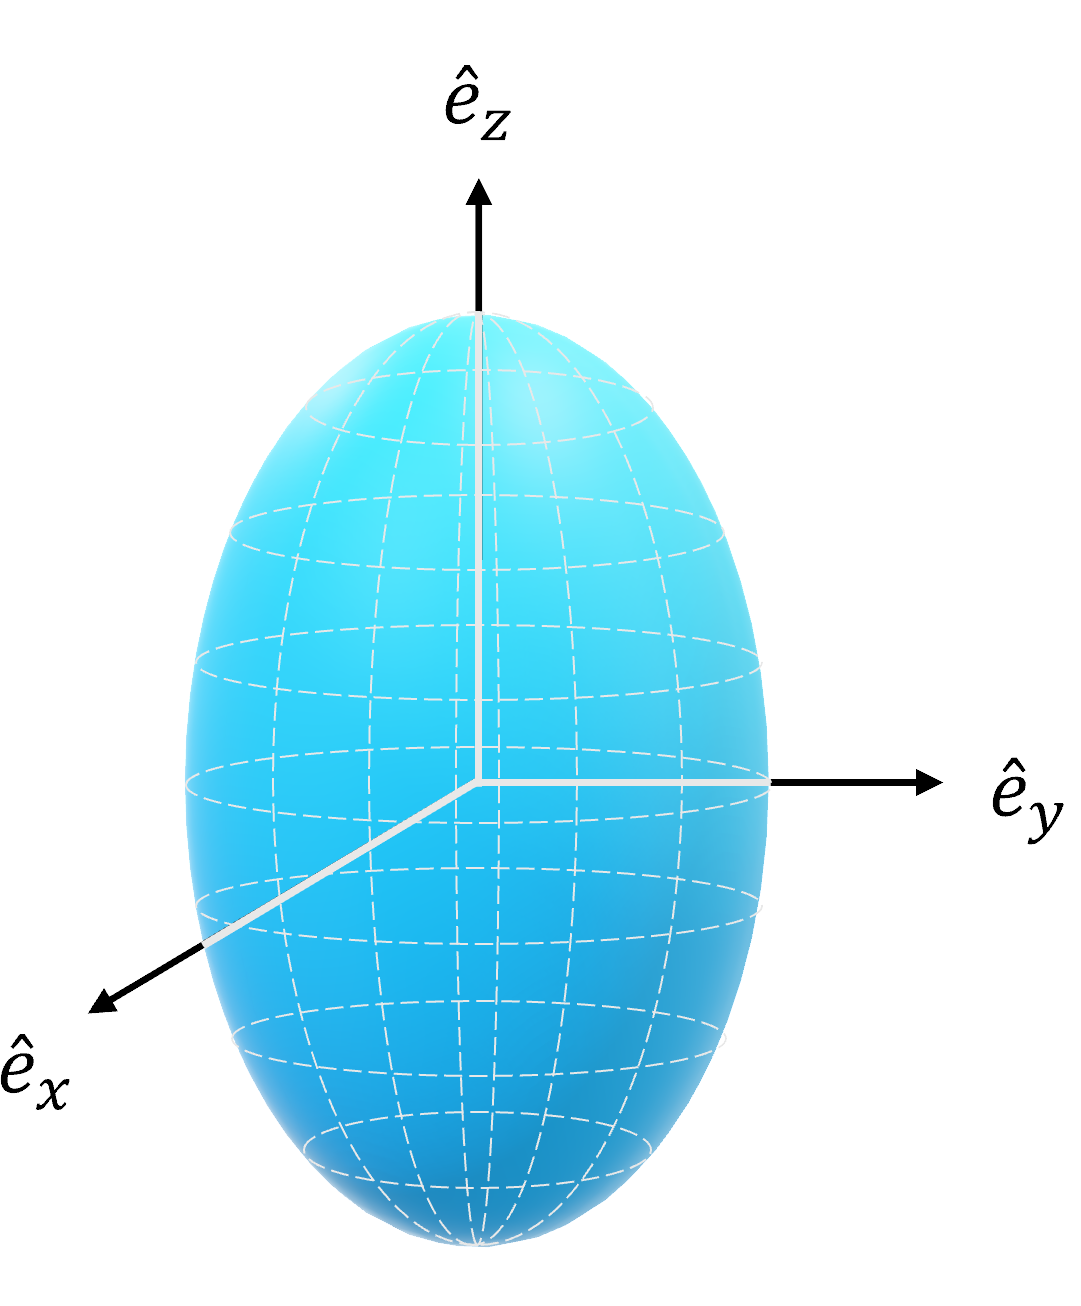
\includegraphics[width=3cm]{../../Figuras/prolato} \label{esf_prolato}}\quad%
	\sidesubfloat[]{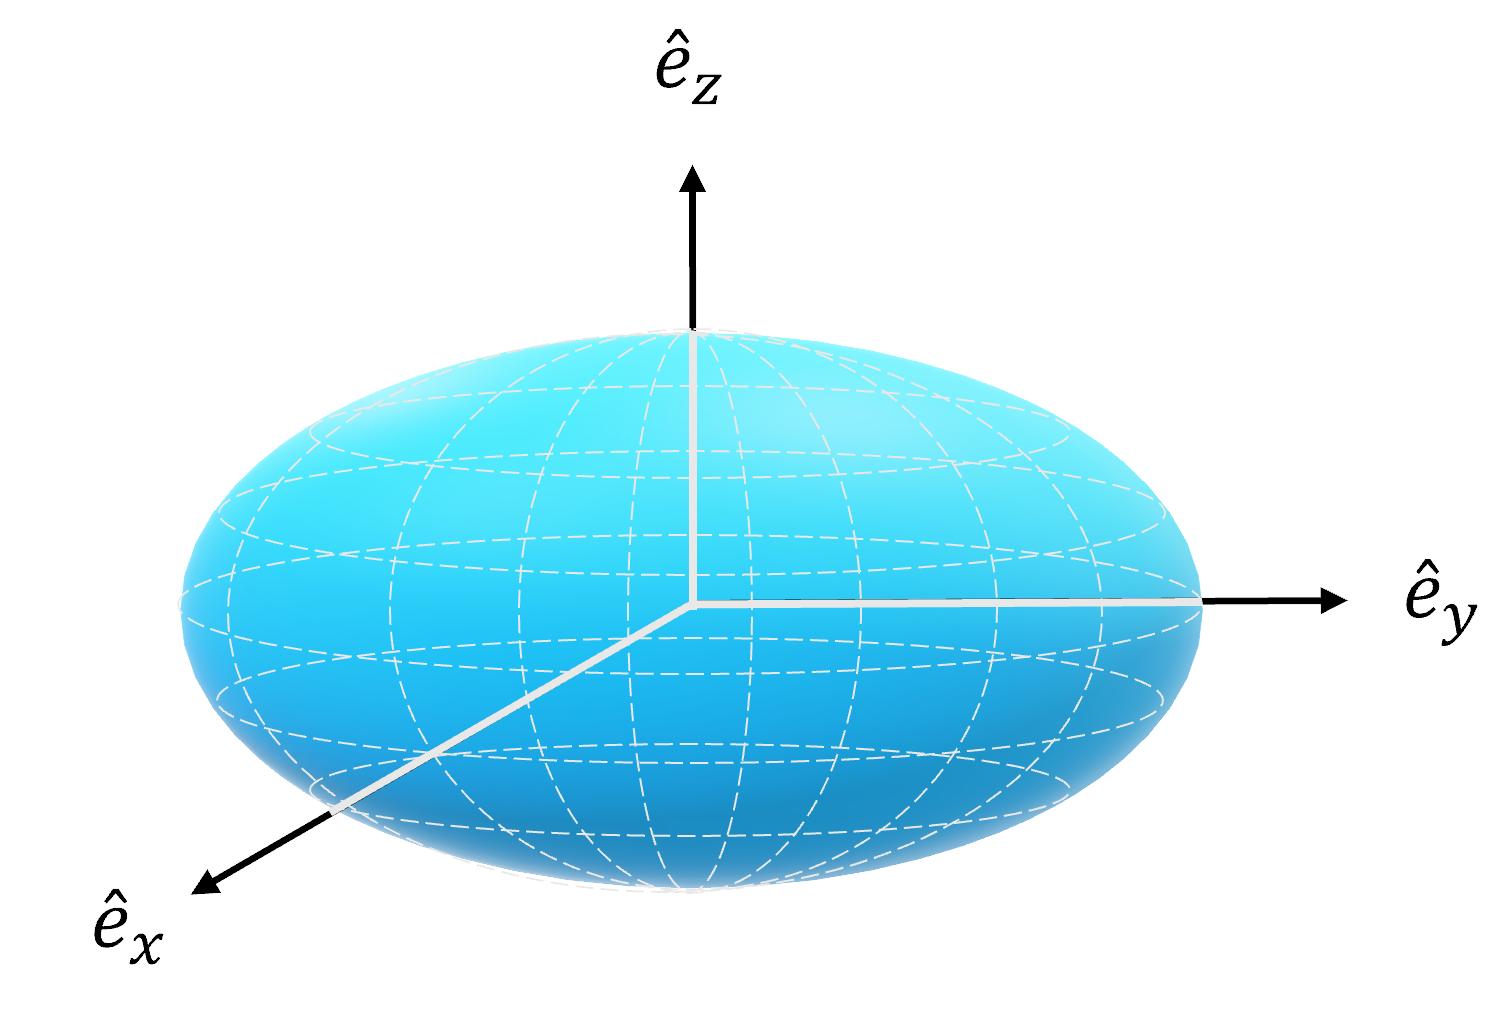
\includegraphics[width=.3\textwidth]{../../Figuras/oblato}\label{esf_oblato}}%
	\caption{Clases especiales de elipsoides. \textbf{a)} Prolato. El eje mayor del elipsoide está orientado en la dirección del eje $\hat{e}_z$. \textbf{b)} Oblato. El eje mayor del elipsoide está orientado en la dirección del eje $\hat{e}_y$.}\label{fig:test}
\end{figure}


	\hypertarget{resultados}{\section{Resultados}}
En esta sección se muestran las secciones transversales para elipsoides oblatos, empleados como una primera aproximación a la forma discoide cóncava de los eritrocitos. Dado el bajo contraste entre los eritrocitos y el medio en el que están inmersos en una muestra real\footnote{El contraste en el índice de refracción entre los eritrocitos y el plasma sanguíneo es relativamente bajo (0.04 - 0.06) \cite{Blood}.}, el esparcimiento de luz es despreciable. Como resultado, el campo que excita a los eritrocitos es, en promedio, igual al campo externo. Además, dado que los eritrocitos están orientados aleatoriamente, se estudia su respuesta óptica promedio considerando que una onda plana ilumina una colección de eritrocitos idénticos y no interactuantes. Por la aleatoridad de los elipsoides considerados, se emplea la respuesta promedio, que considera la excitación de un elipsoide a los largo de sus tres semiejes. De esta forma, las secciones transversales promedio de absorción y esparcimiento se expresan como \cite{Bohren}:
\begin{align*}
	\langle C_{abs}\rangle &= \frac{k}{3} \text{Im}\{\alpha^{(1)}+\alpha^{(2)}+\alpha^{(3)}\},\\
	\langle C_{sca}\rangle &= \frac{k^4}{3(6\pi)} \left(\alpha^{(1)}+\alpha^{(2)}+\alpha^{(3)}\right)^2.
\end{align*}

Para modelar la respuesta electromagnética del material de los elipsoides, se propone emplear el modelo de Drude. Este modelo describe el comportamiento plasmónico de materiales a energías bajas, es decir, aquella dominada por los electrones en la banda de conducción. Al considerar que una colección de electrones no interactuantes entre sí de un material se encuentran bajo la presencia de un campo eléctrico armónico con una frecuencia $\omega$, la expresión de la función dieléctrica dada por el modelo de Drude es \cite{Plasmonics}
\begin{equation} \epsilon(\omega) = 1 - \frac{\omega_p^2}{\omega^2 + i\gamma\omega}, 
\label{Drude}
\end{equation}
donde $\omega_p$ es la frecuencia de plasma y $\gamma$ es la constante fenomenológica de amortiguamiento, ambas características de cada material. A pesar de  que los eritrocitos no están compuestos por materiales dominados por un comportamiento plasmónico en el espectro visible, se emplea el modelo de Drude debido a su dependencia en la frecuencia, lo que permite, al seleccionar los parámetros $\omega_p$ y $\gamma$, un control sobre la respuesta óptica del sistema, resultando adecuado para estudiar la respuesta general y familiarizarse con el problema.\\

Para analizar la respuesta óptica en partículas elipsoidales dentro del régimen cuasiestático al compararlas con la respuesta de una esfera, se emplea inicialmente la función dieléctrica del aluminio dada por el modelo de Drude con los parámetros $\hbar\omega_p=13.142\text{ eV}$ y $\hbar\gamma=0.197\text{ eV}$ \cite{Aluminio}; adicionalmente el medio donde se encuentra el elipsoide está caracterizado por una función dieléctrica $\epsilon_m = 1.77$, que corresponde al de un medio acuoso\footnote{Que podría considerarse como el plasma sanguíneo \cite{Blood}.}. En la Fig. \ref{Contribuciones} se muestra $\langle C_{abs} \rangle$ (línea verde oscuro) y $\langle C_{sca} \rangle$ (línea verde claro) de  un elipse con semiejes $a=1.5\text{ nm}$, $c=1\text{ nm}$, y $\langle C_{abs} \rangle$ (línea roja punteada) y $\langle C_{sca} \rangle$ (línea naranja punteada) de una esfera con radio igual a $1.5\text{ nm}$. Todas las cantidades se muestran
en función de la energía $\hbar\omega$ (eje inferior) y la longitud de onda $\lambda$ (eje superior) de la onda electromagnética incidente. \\
\begin{figure}[h!]
	\sidesubfloat[]{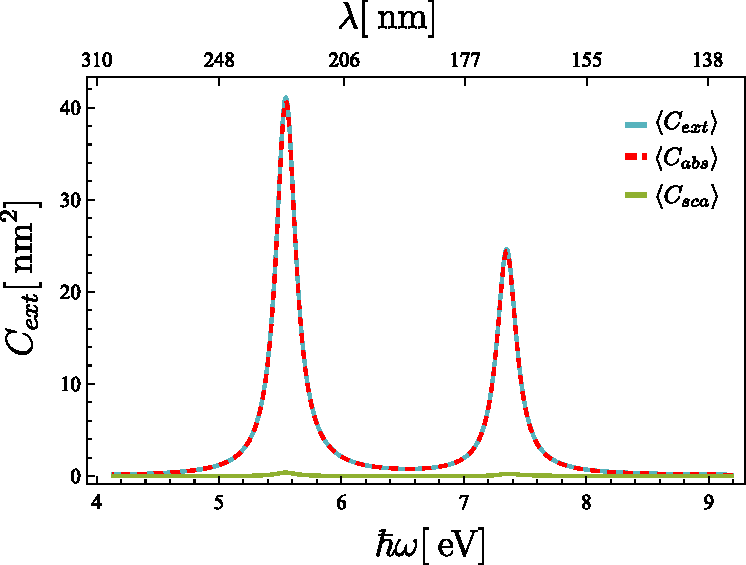
\includegraphics[width=.445\textwidth]{../../Figuras/AlContribuciones3.pdf} \label{Contribuciones}}\quad%
	\sidesubfloat[]{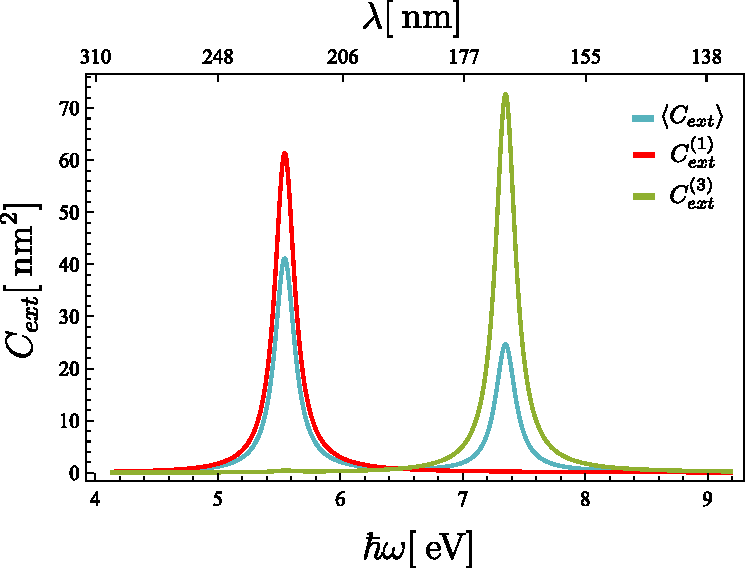
\includegraphics[width=.44\textwidth]{../../Figuras/CextAlbueno.pdf}\label{Cextpromedio}}%
	\caption{Secciones transversales en función de la energía $\hbar\omega$ (eje inferior) y de la longitud de onda $\lambda$ (eje superior) para una partícula elipsoidal oblata de aluminio caracterizada por una función dieléctrica dada por el modelo de Drude ($\hbar\omega_p=13.142\text{ eV}$, $\hbar\gamma=0.197\text{ eV}$), con semiejes $a=b=1.5\text{ nm}$, $c=1\text{ nm}$ e inmersa en un medio acuoso ($\epsilon_m=1.77$). \textbf{a)}~Sección transversal de absorción promedio $\langle C_{ext}\rangle$  del elipsoide (línea verde oscuro) y la esfera (línea violeta punteada) y sección transversal de esparcimiento promedio $\langle C_{abs}\rangle$  del elipsoide (línea verde claro) y la esfera (línea rosa punteada) en escala logarítmica. \textbf{b)} Sección transversal de extinción promedio $\langle C_{ext}\rangle$ del elipsoide (línea azul) y de una esfera de radio igual a 1.5 nm (línea gris punteada), sección transversal de extinción al iluminar al elipsoide con una onda polarizada en la dirección $\hat{e}_x$, $C_{ext}^{(1)}$  (línea roja)  y sección transversal de extinción al iluminar al elipsoide con una onda polarizada en la dirección $\hat{e}_z$ $C_{ext}^{(3)}$  (línea verde).} \label{fig:test}
\end{figure}

A partir de los resultados mostrados en la Fig. \ref{Contribuciones}, se observa que, en partículas dentro del régimen cuasiestático, la absorción domina sobre el esparcimiento en la contribución a la extinción.  La diferencia de magnitudes entre las curvas de absorción y esparcimiento evidencia este comportamiento, ya que la absorción es aproximadamente tres órdenes de magnitud mayor. Como resultado, la curva de extinción es esencialmente la misma que la de absorción. Debido al fuerte contraste entre ambas contribuciones, los análisis posteriores se centran exclusivamente en las secciones transversales de extinción, dado que el esparcimiento es despreciable.\\

El análisis de las diferencias entre $\langle C_{ext}\rangle$ y  las secciones transversales de extinción obtenidas al iluminar la partícula con una onda polarizada en una única dirección, se presenta en la Fig. \ref{Cextpromedio}. En esta figura se muestra $\langle C_{ext}\rangle$ (línea azul), $C_{ext}^{(1)}$ (línea roja) y $C_{ext}^{(3)}$ (línea verde) de un elipsoide y  $\langle C_{ext}\rangle$ (línea gris punteada) de una esfera. Las cantidades se muestran en función de $\hbar\omega$ (eje inferior) y de $\lambda$ (eje superior) de la onda electromagnética incidente. Estos cálculos corresponden a un sistema con las mismas características que el de la Fig. \ref{Contribuciones}. Se observa que debido a la geometría,
$\langle C_{ext}\rangle$ del elipsoide presenta dos máximos, los cuales coinciden con las frecuencias de los máximos de $C_{ext}^{(1)}$ y $C_{ext}^{(3)}$ que se encuentran hacia el rojo y al azul, respectivamente, de la frecuencia de resonancia correspondiente a una partícula esférica. Esto muestra que las secciones transversales promedio son útiles para representar el efecto de iluminar una partícula elipsoidal con una onda electromagnética polarizada en la dirección de cualquiera de sus tres ejes principales, ya que lo que cambia es el valor nominal de los máximos en la sección transversal promedio, más no su localización espectral. \\

Las siguientes figuras presentan los cálculos de las secciones tranversales de extinción promedio  $\langle C_{ext}\rangle$ considerando nanopartículas elipsoidales oblatas cuya función dieléctrica está caracterizada por el modelo de Drude para aluminio \cite{Aluminio} y por datos experimentales para plata \cite{Plata}, oro \cite{Plata}, bismuto \cite{Bismuto} y  óxido de magnesio \cite{MgO}.


\subsection*{Aluminio y plata}
En la Fig. \ref{aluminioplataAR} se muestra $\langle C_{ext}\rangle$ en función de $\hbar\omega$ (eje inferior) y de  $\lambda$ (eje superior) de la onda electromagnética incidente en nanopartículas elipsoidales oblatas de aluminio (AlNPs) [Fig. \ref{aluminioAR}] y plata (AgNPs) [Fig.~\ref{plataAR}]. La función dieléctrica para el aluminio está dada por el modelo de Drude con parámetros $\hbar\omega_p=13.142\text{ eV}$, $\hbar\gamma=0.197\text{ eV}$ \cite{Aluminio}, mientras que para la plata  está dada a partir de los datos experimentales reportados por Johnson y Christy \cite{Plata}. Se realizan los cálculos para partículas elipsoidales con razón de aspecto AR=2 y con semiejes de tamaño desde 1 nm a 2.5 nm, en pasos de 0.5 nm; cada caso se identifica con el código de color mostrado en la gráfica. Además, se incluyen los cálculos para una partícula esférica con radio igual a $2 \text{ nm}$ (línea gris punteada). Todas las partículas están  inmersas en un medio acuoso con $\epsilon_m=1.77$. Como parte del análisis, se muestra debajo de las gráficas la función dieléctrica del aluminio, obtenida a partir de la Ref. \cite{Aluminio}, junto con la de la plata, en donde los puntos corresponden a datos experimentales \cite{Plata}, y las líneas continuas representan la interpolación realizada para dichos datos.
\\

\begin{figure}[h!]
	\sidesubfloat[]{\includegraphics[width=.44\textwidth]{../../Figuras/Al1} \label{aluminioAR}}\quad%
	\sidesubfloat[]{\includegraphics[width=.44\textwidth]{../../Figuras/Ag1}\label{plataAR}}%
	\caption{Secciones transversales de extinción promedio en función de la energía (eje inferior) y de la longitud de onda (eje superior) de la onda electromagnética incidente para una partícula elipsoidal oblata inmersa en un medio acuoso ($\epsilon_m=1.77$).  Las partículas poseen AR=2, excepto en el caso de la línea gris punteada en el que AR=1 (partícula esférica). Además, las partículas están caracterizadas por una función dieléctrica dada por  \textbf{a)} el modelo de Drude para el aluminio con parámetros $\hbar\omega_p=13.142\text{ eV}$ y $\hbar\gamma=0.197\text{ eV}$ \cite{Aluminio} y \textbf{b)} datos experimentales correspondientes a la plata obtenidos de la Ref. \cite{Plata}. Debajo de las gráficas se muestra la función dieléctrica del \textbf{a)} aluminio dada por el modelo de Drude obtenida a partir de la Ref. \cite{Aluminio} y \textbf{b)} plata obtenida a partir de la Ref. \cite{Plata}; en ambos casos se indica en azul la parte real de la función dieléctrica y en rojo la parte imaginaria. La línea recta que une los puntos experimentales en \textbf{b)}  fue obtenida mediante una interpolación.}\label{aluminioplataAR}
\end{figure}
A partir de los resultados de la Fig. \ref{aluminioplataAR}, se observa que al aumentar el tamaño de la partícula mientras se mantiene constante AR, la localización espectral de las resonancias no cambia pero su valor nominal aumenta. Se identifican dos máximos locales en $\langle C_{ext}\rangle$,  los cuales corresponden a las frecuencias en las que $C_{ext}^{(1)}$ y $C_{ext}^{(3)}$ se maximizan. En ambos casos se observa que el corrimiento  de la resonancia no es simétrico respecto al de la esfera, para $C_{ext}^{(1)}$, las resonancias presentan un corrimiento hacia el rojo de $\Delta\lambda=$44 nm (1.11 eV) para las AlNPs y $\Delta\lambda=$51 nm (0.38 eV) para las AgNPs. Para $C_{ext}^{(3)}$, las resonancias presentan un corrimiento hacia el azul de $\Delta\lambda=$55 nm (2.33 eV) para AlNPs y $\Delta\lambda=$39 nm (0.36 eV) para las AgNPs. Es decir, este corrimiento depende del material. \\

El efecto de la variación de la razón de aspecto en la sección transversal de extinción promedio en AlNPs y AgNPs inmersas en un medio acuoso con $\epsilon_m=1.77$ se muestra en la Fig. \ref{aluminioplatacc}. En esta figura, las partículas elipsoidales se consideran con AR entre 1.5 a 2.25, con incrementos 0.25 y con un semieje menor fijo de $c=1\text{ nm}$ y también se incluye $\langle C_{ext}\rangle$ para una partícula esférica con radio igual a $1\text{ nm}$.\\


\begin{figure}[h!]
	\sidesubfloat[]{\includegraphics[width=.44\textwidth]{../../Figuras/Al2} \label{aluminioc}}\quad%
	\sidesubfloat[]{\includegraphics[width=.44\textwidth]{../../Figuras/Ag2}\label{platac}}%
	\caption{Secciones transversales de extinción promedio en función de la energía (eje inferior) y de la longitud de onda (eje superior) de la onda electromagnética incidente para una partícula elipsoidal oblata inmersa en un medio acuoso ($\epsilon_m=1.77$). Las partículas  poseen un semieje menor de tamaño $c=1$ nm y presentan diferentes AR cuyo código de color se muestra en la gráfica. Además, las partículas están caracterizadas por una función dieléctrica dada por  \textbf{a)} el modelo de Drude para el aluminio ($\hbar\omega_p=13.142\text{ eV}$, $\hbar\gamma=0.197\text{ eV}$) y \textbf{b)} datos experimentales correspondientes a la plata obtenidos de la Ref. \cite{Plata}. Debajo de las gráficas se muestra la función dieléctrica del \textbf{a)} aluminio dada por el modelo de Drude obtenida a partir de la Ref. \cite{Aluminio} y \textbf{b)} plata obtenida a partir de la Ref. \cite{Plata}; en ambos casos se indica en azul la parte real de la función dieléctrica y en rojo la parte imaginaria. La línea recta que une los puntos experimentales en \textbf{b)}  fue obtenida mediante una interpolación.} \label{aluminioplatacc}
\end{figure} 

 En la Fig. \ref{aluminioplatacc} se observa que conforme la relación de aspecto se aproxima a la unidad, hay un corrimiento de las frecuencias asociadas a $\langle C_{ext}\rangle$ máximas hacia la frecuencia de resonancia asociada a una partícula esférica. Esta frecuencia de resonancia corresponde a $\lambda=201\text{ nm}$ (6.17 eV) para el aluminio y $\lambda=383\text{ nm}$ (3.24 eV) para la plata. Además, tanto en el aluminio como en la plata, se observa que al aumentar la relación de aspecto y la longitud del eje mayor, el valor nominal de  $\langle C_{ext}\rangle$ también aumenta. Esto se debe a que hay una mayor cantidad de material y por tanto más electrones, por lo que los efectos de absorción aumentan, lo que, en consecuencia, aumenta la extinción. En las AlNPs y AgNPs es posible observar dos resonancias debido a que en las frecuencias en las que se presentan, ambos materiales, el aluminio y la plata, presentan baja absorción.




\subsection*{Oro y bismuto}
De forma análoga al análisis en la variación de los parámetros geométricos de las AlNPs y AgNPs, se muestra en la Fig. \ref{oro} la respuesta óptica variando estos parámetros (semieje mayor y razón de aspecto) considerando una función dieléctrica donde se observan contribuciones no descritas por el modelo de Drude.\footnote{Estas contribuciones provienen de electrones ligados \cite{Plasmonics}.} En particular, en la Fig. \ref{oroAR} se grafica $\langle C_{ext}\rangle$ en función de $\hbar\omega$ (eje inferior) y de $\lambda$ (eje superior) para nanopartículas elipsoidales oblatas de oro (AuNPs) de distintos tamaños que conservan la razón de aspecto de AR=2. Para complementar el análisis, se muestra debajo de esta gráfica la función dieléctrica del oro donde los puntos representan datos experimentales \cite{Plata} y las líneas continuas corresponden a la interpolación empleada para este conjunto de datos. En la Fig. \ref{oroAR} se consideran partículas con relación de aspecto AR$=2$ con radio desde 1  nm a 2.5 nm, con incrementos de 0.5 nm; cada caso se identifica con el código de color mostrado en la gráfica respectiva. También se considera una partícula con relación de aspecto AR$=1$ y semiejes $a=2$ nm (línea gris punteada), que representa a una partícula esférica. Por otro lado, en la Fig. \ref{oroc} se consideraron partículas con relación de aspecto variable AR=1.5 (línea roja), AR=1.75 (línea naranja), AR=2 (línea verde) y AR=2.25 (línea azul) que presentan valores en su semieje menor $c=1\text{ nm}$. Asimismo, se considera una partícula esférica con radio igual a $1\text{ nm}$ (línea gris).\\
\begin{figure}[h]
	\sidesubfloat[]{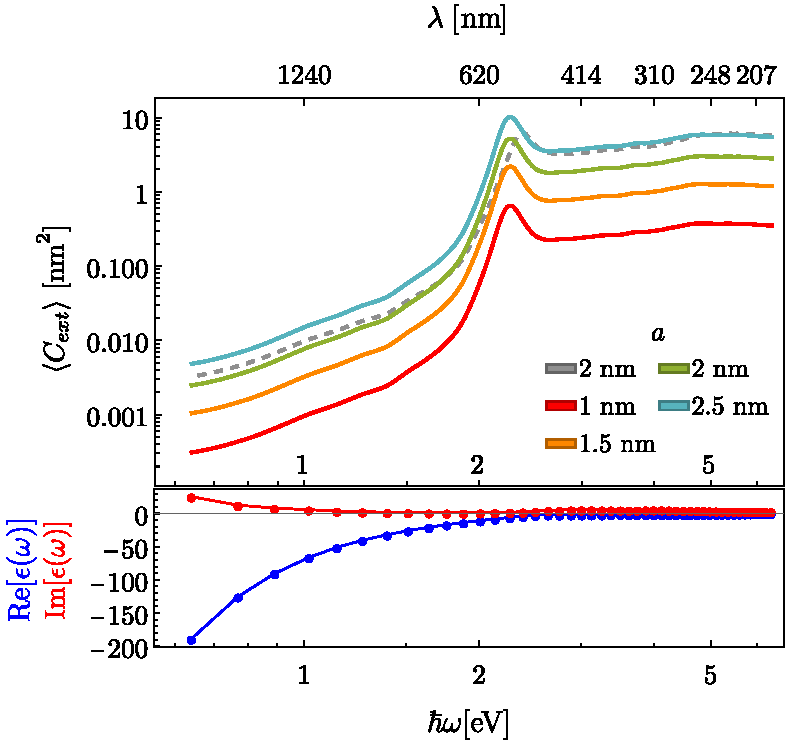
\includegraphics[width=.445\textwidth]{../../Figuras/Au2.pdf} \label{oroAR}}\quad%
	\sidesubfloat[]{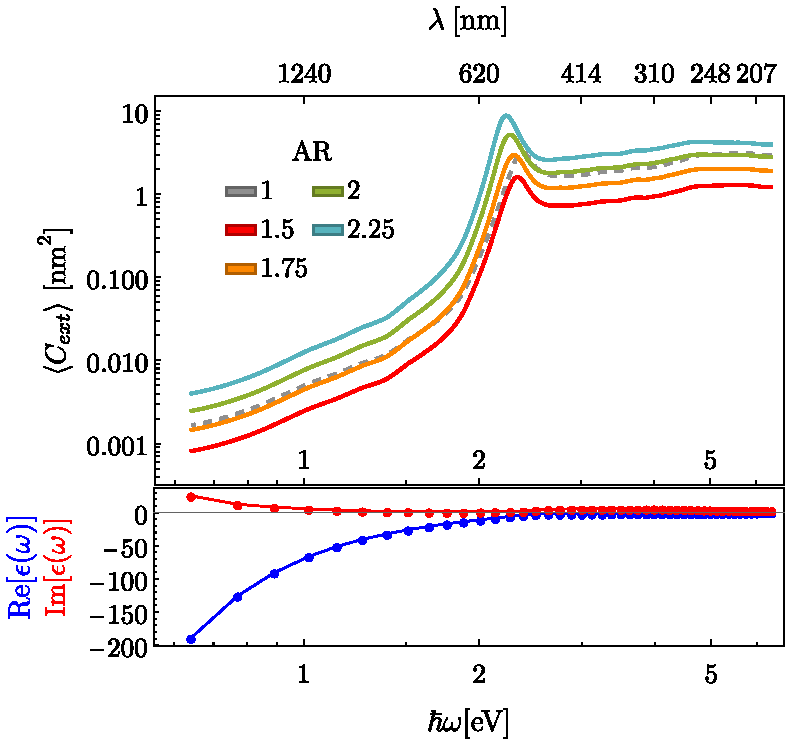
\includegraphics[width=.44\textwidth]{../../Figuras/Au.pdf}\label{oroc}}%
	\caption{Secciones transversales de extinción promedio en función de la energía (eje inferior) y de la longitud de onda (eje superior) para una partícula elipsoidal oblata de oro inmersa en un medio acuoso con $\epsilon_m=1.77$, y cuyo índice de refracción complejo fue obtenido a partir de datos experimentales de la Ref. \cite{Plata}. Debajo de las gráficas se muestra la función dieléctrica del oro obtenida a partir de la Ref. \cite{Plata} (parte real en azul, parte imaginaria en rojo). La línea recta que une los puntos experimentales fue obtenida mediante una interpolación. \textbf{a)} AuNPs con AR=2, excepto en el caso de una esfera (línea gris punteada) donde AR=1. \textbf{b)} AuNPs con semieje menor $c=1$ nm.}\label{oro}
\end{figure}

En contraste con el aluminio y la plata, para el oro se observa sólo una excitación plasmónica en $\lambda=$ 522 nm (2.38 eV). Esta excitación presenta un corrimiento hacia el rojo respecto de la de la esfera en $\lambda=$ 547 nm (2.27 eV) y se esperaría que existiera otra con un corrimiento hacia el azul es decir, a frecuencias mayores, más no la hay como sí se observó en el análisis de la Fig. \ref{aluminioplataAR}. Esto se atribuye a la fuerte absorción del oro a energías altas, lo que suprime resonancias atribuidas a contribuciones no descritas por el modelo de Drude en los datos experimentales.\footnote{En particular de contribuciones dieléctricas descritas por el modelo de Lorentz \cite{Plasmonics}.} Por otro lado, se observa que para AR=2.25, la resonancia se encuentra en $\lambda=$ 556 nm (2.23~eV), mientras que para AR=1.5, el caso calculado más cercano al de una esfera, la resonancia se encuentra en $\lambda=$~522~nm (2.33~eV), es decir, la AR reproduce el caso de una esfera en su respuesta espectral cuando tiende a la unidad, resultado que sigue las tendencias observadas en las AlNPs y AgNPs.\\

En los casos anteriores se analizó el aluminio, modelando la respuesta óptica por el modelo de Drude, así como se analizaron metales nobles como la plata y el oro. Ahora, con el objetivo de aproximarse a las propiedades ópticas de los eritrocitos, en la Fig. \ref{bismuto} se presentan las secciones transversales de extinción promedio en función de la energía (eje inferior) y la longitud de onda (eje superior) para nanopartículas elipsoidales oblatas de bismuto (BiNPs). Este material, al ser un semimetal, exhibe en ciertas regiones espectrales un comportamiento más similar al de los eritrocitos que los materiales previamente estudiados. Como complemento, debajo de las gráficas se muestra la función dieléctrica del bismuto obtenida de datos experimentales reportados por Hagemann et al. \cite{Bismuto}. En la Fig. \ref{bismutoAR} se consideraron partículas con  AR$=2$  y en la Fig. \ref{bismutoc} se consideraron partículas con relación de aspecto variable desde 1.5 hasta 2.25, con incrementos de 0.25.  \\

\begin{figure}[]
	\sidesubfloat[]{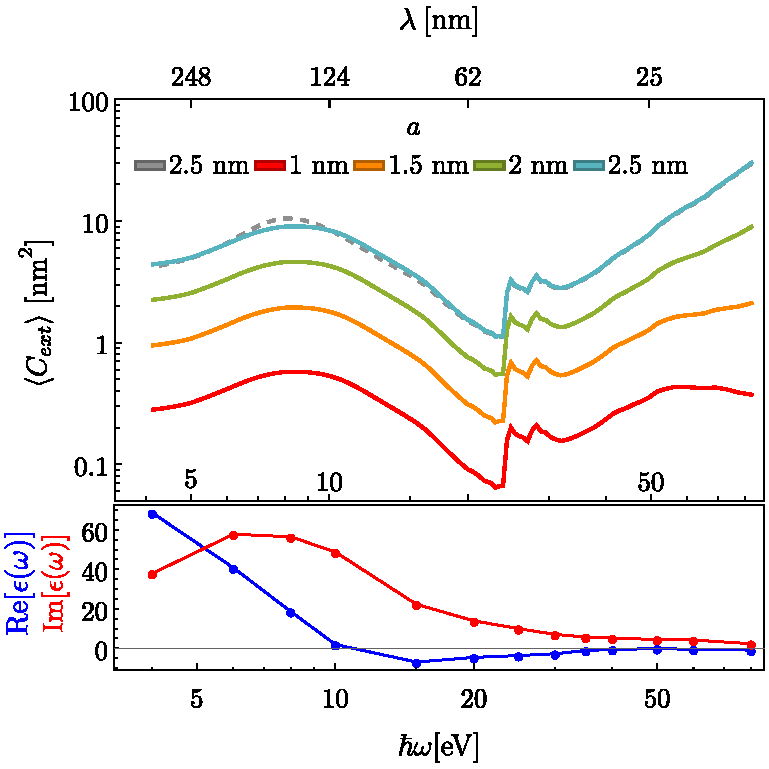
\includegraphics[width=.445\textwidth]{../../Figuras/Bi2} \label{bismutoAR}}\quad%
	\sidesubfloat[]{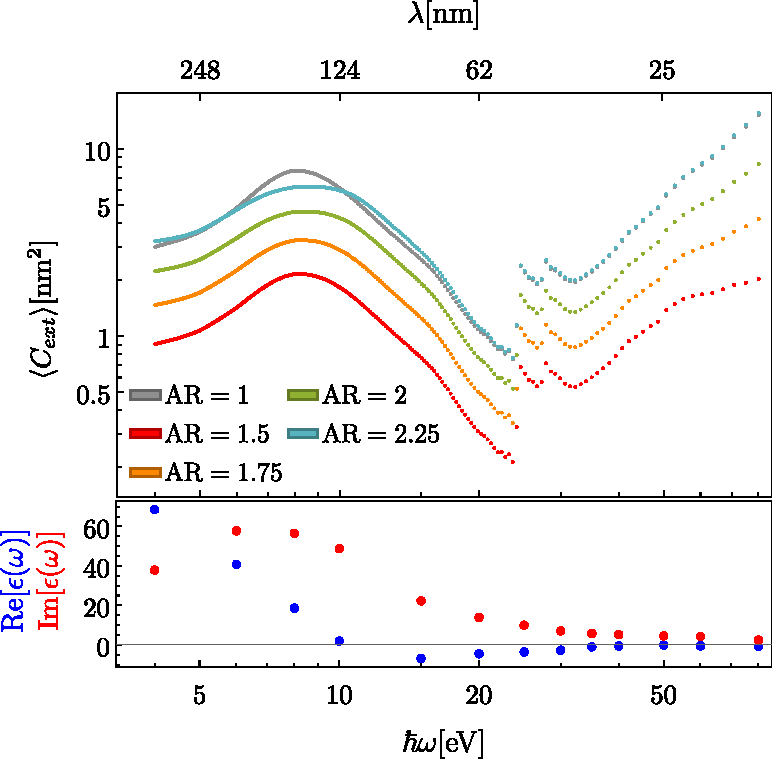
\includegraphics[width=.44\textwidth]{../../Figuras/Bi}\label{bismutoc}}%
	\caption{Secciones transversales de extinción promedio  en función de la energía (eje inferior) y de la longitud de onda (eje superior) para una partícula elipsoidal oblata de bismuto inmersa en un medio acuoso con $\epsilon_m=1.77$, y cuyo índice de refracción complejo fue obtenido a partir de datos experimentales de la Ref. \cite{Bismuto}. Debajo de las gráficas se muestra la función dieléctrica del oro obtenida a partir de la Ref. \cite{Plata} (parte real en azul, parte imaginaria en rojo). La línea recta que une los puntos experimentales fue obtenida mediante una interpolación. \textbf{a)} BiNPs con AR=2, excepto en el caso de una esfera (línea gris punteada) donde AR=1. \textbf{b)} BiNPs con semieje menor $c=1$ nm.}\label{bismuto}
\end{figure}

En ambas figuras se observan frecuencias de resonancia alrededor de $\lambda=147$ nm (8.44 eV), que se encuentran hacia el azul de la frecuencia de resonancia en $\lambda=154$ nm (8.03 eV) correspondiente a una nanopartícula esférica y de manera similar al caso del oro, se esperaría que existiera otra resonancia hacia el rojo de la de la esfera. También se observa un aumento de $\langle C_{ext}\rangle$ a partir de $\lambda=50$ nm (24.81 eV) y la presencia de dos máximos locales en $\lambda=50$ nm (24.81 eV) y $\lambda=44$ nm (28.19 eV), los cuales se atribuyen a procesos de absorción de contribuciones no descritas por el modelo de Drude en los datos experimentales. Como en los casos anteriores, se observa que al aproximar AR a la unidad, se recupera la frecuencia de resonancia correspondiente a una nanopartícula esférica. Además, en el caso del bismuto (que es un semimetal), las excitaciones plasmónicas están menos definidas que en el caso de los materiales plasmónicos. Esto es más evidente al comparar la anchura a media altura (FWHM por sus siglas en inglés) pues, en el caso del bismuto se observa un FHWM = 68.54 nm (3.64 eV), mientras que en el aluminio FWHM = 8.85 nm (0.18 eV). La diferencia de los valores del FWHM se explica debido a la fuerte absorción del bismuto en el rango de frecuencias estudiado.





\subsection*{Óxido de magnesio (MgO)}
En la Fig. (\ref{mgo}) se muestra $\langle C_{ext}\rangle$ en función de la energía (eje inferior) y de la longitud de onda (eje superior) para un material dieléctrico: el óxido de magnesio (MgO). Se emplearon los datos experimentales reportados por Stephens y Malitson \cite{MgO}. De la misma forma que con los materiales anteriores, se consideraron partículas con relación de aspecto AR$=2$ con radio desde 1  nm a 2.5 nm, con incrementos de 0.5 nm, con su respectivo código de color indicado en la gráfica [ver Fig. \ref{mgoc}] y en la Fig. \ref{mgoAR} se consideraron partículas con AR variable.  Como complemento, se muestra debajo de ésta gráfica  la función dieléctrica del óxido de magnesio donde los puntos representan datos experimentales obtenidos a partir de la Ref. \cite{MgO} y las líneas continuas corresponden a la interpolación empleada para dicho conjunto de datos.

\begin{figure}[H]
	\sidesubfloat[]{\includegraphics[width=.445\textwidth]{../../Figuras/MgO1} \label{mgoc}}\quad%
	\sidesubfloat[]{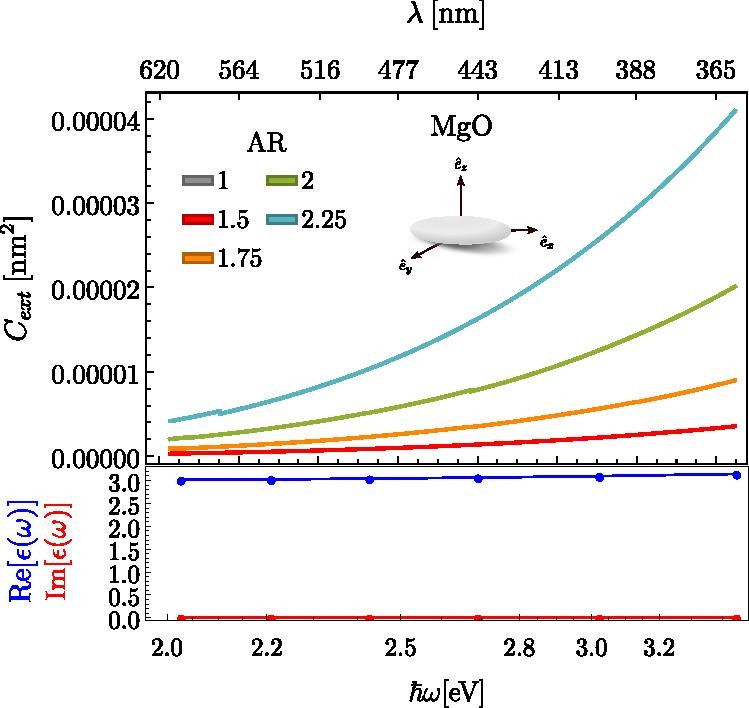
\includegraphics[width=.44\textwidth]{../../Figuras/MgO2}\label{mgoAR}}%
	\caption{Secciones transversales de extinción promedio en función de la energía (eje inferior) y de la longitud de onda (eje superior) para una partícula elipsoidal oblata de óxido de magnesio inmersa en un medio acuoso ($\epsilon_m=1.77$). Debajo de las gráficas se muestra la función dieléctrica del óxido de magnesio obtenida a partir de la Ref. \cite{MgO} (parte real en azul, parte imaginaria en rojo). La línea recta que une los puntos experimentales fue obtenida mediante una interpolación. \textbf{a)} MgONPs con AR=2, excepto en el caso de una esfera (línea gris punteada) donde AR=1. \textbf{b)}  MgONPs con semieje menor $c=1$ nm.}\label{mgo}
\end{figure}

En las Figs. \ref{mgoc} y \ref{mgoAR} se observa que $\langle C_{ext}\rangle$ tiene un comportamiento creciente y no se observan resonancias plasmónicas debido a la naturaleza dieléctrica del óxido de magnesio.








\section{Conclusiones}

En este trabajo se estudió la solución analítica del problema de esparcimiento de luz por partículas elipsoidales arbitrarias en la aproximación cuasiestática, analizando las secciones transversales de extinción, absorción y esparcimiento. Además, se estudió el comportamiento del esparcimiento de luz por un elipsoide centrado en el origen dentro de este mismo régimen, comparando los resultados con la respuesta de esferas calculadas también en el límite cuasiestático.\\

Se encontró que, en el régimen cuasiestático, la absorción es la contribución predominante en la extinción para nanopartículas elipsoidales oblatas de aluminio, mientras que el esparcimiento resulta despreciable. En el rango en el que el modelo de Drude se adapta al comportamiento de los materiales, se identificaron dos resonancias plasmónicas desplazadas hacia el rojo y el azul respecto a la frecuencia de resonancia observada en una nanopartícula esférica. Para materiales más realistas, se determinó que es necesario incluir contribuciones adicionales a las plasmónicas, como las descritas por el modelo de Lorentz.




\printbibliography



%----------------------------------------------------------------------------------------
\end{document}
